%% LyX 2.1.1 created this file.  For more info, see http://www.lyx.org/.
%% Do not edit unless you really know what you are doing.
\documentclass[11pt,english,australian]{report}
\usepackage{mathptmx}
\renewcommand{\familydefault}{\rmdefault}
\usepackage[T1]{fontenc}
\usepackage[latin9]{inputenc}
\usepackage[a4paper]{geometry}
\geometry{verbose,tmargin=25mm,bmargin=25mm,lmargin=40mm,rmargin=25mm}
\usepackage{fancyhdr}
\pagestyle{fancy}
\setcounter{secnumdepth}{3}
\setcounter{tocdepth}{3}
\setlength{\parskip}{\smallskipamount}
\setlength{\parindent}{0pt}
\synctex=-1
\usepackage{color}
\definecolor{shadecolor}{rgb}{0.97265625, 0.9140625, 0.61328125}
\usepackage{babel}
\usepackage{array}
\usepackage{varioref}
\usepackage{refstyle}
\usepackage{float}
\usepackage{framed}
\usepackage{textcomp}
\usepackage{pdfpages}
\usepackage{graphicx}
\usepackage{setspace}
\usepackage{nomencl}
% the following is useful when we have the old nomencl.sty package
\providecommand{\printnomenclature}{\printglossary}
\providecommand{\makenomenclature}{\makeglossary}
\makenomenclature
\onehalfspacing
\usepackage{nameref}

\makeatletter

%%%%%%%%%%%%%%%%%%%%%%%%%%%%%% LyX specific LaTeX commands.

\AtBeginDocument{\providecommand\tabref[1]{\ref{tab:#1}}}
\AtBeginDocument{\providecommand\figref[1]{\ref{fig:#1}}}
\AtBeginDocument{\providecommand\chapref[1]{\ref{chap:#1}}}
\AtBeginDocument{\providecommand\secref[1]{\ref{sec:#1}}}
\AtBeginDocument{\providecommand\lstref[1]{\ref{lst:#1}}}
\AtBeginDocument{\providecommand\algref[1]{\ref{alg:#1}}}
\providecommand{\LyX}{L\kern-.1667em\lower.25em\hbox{Y}\kern-.125emX\@}
%% Because html converters don't know tabularnewline
\providecommand{\tabularnewline}{\\}
%% A simple dot to overcome graphicx limitations
\newcommand{\lyxdot}{.}

\floatstyle{ruled}
\newfloat{algorithm}{tbp}{loa}[chapter]
\providecommand{\algorithmname}{Algorithm}
\floatname{algorithm}{\protect\algorithmname}
\floatstyle{ruled}
\newfloat{listing}{tbp}{lol}[chapter]
\providecommand{\listingname}{Listing}
\floatname{listing}{\protect\listingname}
\RS@ifundefined{subref}
  {\def\RSsubtxt{section~}\newref{sub}{name = \RSsubtxt}}
  {}
\RS@ifundefined{thmref}
  {\def\RSthmtxt{theorem~}\newref{thm}{name = \RSthmtxt}}
  {}
\RS@ifundefined{lemref}
  {\def\RSlemtxt{lemma~}\newref{lem}{name = \RSlemtxt}}
  {}


%%%%%%%%%%%%%%%%%%%%%%%%%%%%%% Textclass specific LaTeX commands.
\usepackage{enumitem}		% customizable list environments
\newlength{\lyxlabelwidth}      % auxiliary length 

%%%%%%%%%%%%%%%%%%%%%%%%%%%%%% User specified LaTeX commands.
\usepackage[novbox]{pdfsync}

\usepackage{csvsimple}

% acronyms
\usepackage{acronym}

% a priori italics
\newcommand\apriori{\textit{a priori}}

% use instead of standard natbib to compress conecutive references
\usepackage[numbers, sort&compress]{natbib}

% capitalise references
\renewcommand{\figref}{\Figref}
\renewcommand{\tabref}{\Tabref}
\renewcommand{\chapref}{\Chapref}
\renewcommand{\secref}{\Secref}

% automatically number all display equations
\renewcommand\[{\begin{equation}}
\renewcommand\]{\end{equation}}

% no paragraph gaps in lists
\setlist{noitemsep}

% format captions
\usepackage[labelfont=bf]{caption}
\captionsetup[table]{singlelinecheck=off,justification=justified} 

% equations use dashed numbering
\makeatletter
\long\def\theequation{\ifnum \c@chapter > \z@ \thechapter --\fi \@arabic \c@equation}

% all headings same, (no difference for chapter beginnings)
\let\ps@plain\ps@fancy
\makeatother

% rename nomenclature
 \renewcommand{\nomname}{List of Symbols}

% chapter title spacing
\usepackage{titlesec}
\titleformat{\chapter}[hang]{\normalfont\Huge\bfseries}{\chaptertitlename \enspace \thechapter :}{20pt}{}{}
\titlespacing*{\chapter}{0pt}{-1cm}{0.5cm}

\clubpenalty=9999
\widowpenalty=9999

\@ifundefined{showcaptionsetup}{}{%
 \PassOptionsToPackage{caption=false}{subfig}}
\usepackage{subfig}
\makeatother

\usepackage{listings}
\addto\captionsaustralian{\renewcommand{\lstlistingname}{Listing}}
\addto\captionsenglish{\renewcommand{\algorithmname}{Algorithm}}
\addto\captionsenglish{\renewcommand{\listingname}{Listing}}
\addto\captionsenglish{\renewcommand{\lstlistingname}{Listing}}
\renewcommand{\lstlistingname}{Listing}

\begin{document}
\begin{titlepage}

\noindent \begin{center}
\includegraphics[width=0.1\paperwidth+0.1\paperheight]{fig/JCU_Logo_RGB}
\par\end{center}

\noindent \begin{center}
{\Huge{}College of Science, Technology and Engineering}
\par\end{center}{\Huge \par}

\noindent \begin{center}
{\LARGE{}EG4012}\\
{\LARGE{}Electrical and Electronic Engineering}
\par\end{center}{\LARGE \par}

\noindent \begin{center}
{\Huge{}Evaluation of Speech Enhancement and Practical Speech Enhancement
in Babble Using Phoneme-Dependent Non-negative Matrix Factorisation}
\par\end{center}{\Huge \par}

\noindent \begin{center}
{\huge{}Ashley Gillman}
\par\end{center}{\huge \par}

\begin{doublespace}
\noindent \begin{center}
{\Large{}Thesis submitted to the School of Engineering \& Physical
Sciences in partial fulfilment of the requirements for the degree
of}
\par\end{center}{\Large \par}
\end{doublespace}

\noindent \begin{center}
{\huge{}Bachelor of Engineering with Honours (Electrical and Electronic
Engineering)}
\par\end{center}{\huge \par}

\noindent \begin{center}
{\Large{}10 October 2014}
\par\end{center}{\Large \par}

\end{titlepage}


\lhead{Gillman}


\rhead{Speech Enhancement and Evaluation}


\cfoot{}% remove centered page no.}


\rfoot{\fancyplain{\thepage}{\thepage}}

\pagenumbering{roman}

\begin{abstract}
Speech enhancement is an important field in modern electronics, finding
many applications from hearing aids to enhancing audio/visual recordings
and automated speech recognisers in commercial products. These can
range from mobile phones to modern televisions and automobile electronics.
A variety of techniques are available to measure speech enhancement.
These fall into three categories: (1) those for measuring speech enhancement
for a human recogniser; (2) those for measuring speech enhancement
for a machine recogniser; and (3) those measuring speech enhancement
using purely statistical methods. However, when an enhancement algorithm
is proposed it is often measured by techniques from only one of those
categories. Due to there being fundamental differences from a human
listener to a machine listener, it is hypothesised that the use of
a variety of enhancement measures is necessary to properly measure
the performance of an enhancement algorithm. Results indicated that
the hypothesis was true, and that it is possible for a speech enhancement
method that performs well for a machine recogniser to perform poorly
for a human recogniser, and vice-versa. Therefore, it is important
to encapsulate a variety of measures in testing. The recommended tests
include PESQ, ASR performance, statistical measures such as segmental
SNR and where possible, MOS.

Investigations were also performed into the effects of varying the
number of sentences used for training. It was found that there was
no correlation, and that varying training did not effect the average
results, however it did effect the variance and therefore reliability
of results, if undertrained. Adequate training was found to be 10
to 20 utterances. Additionally, it was found that training using utterances
was suboptimal. This showed promise for the third research area, which
investigated an alternative training to utterances.

The proposed algorithm training modification was a phoneme-dependent
modification to existing non-negative matrix factorisation algorithms.
This algorithm was found to provide better accuracy for machine recognisers,
especially so under in-car noise conditions. The changes did not improve
human intelligibility on average, but did perform more consistently,
being less likely to distort speech. The system showed capability
of performing well for in-car electronics, such as for voice-controlled
navigational electronics or car radios.\end{abstract}



\tableofcontents{}


\chapter*{Statement of Access}

\selectlanguage{english}%
\addcontentsline{toc}{chapter}{Statement of Access}

\selectlanguage{australian}%
I, the undersigned, author of this work, understand that James Cook
University may make this thesis available for use within the University
Library and, via the Australian Digital Theses network, for use elsewhere.

I understand that, as an unpublished work, a thesis has significant
protection under the Copyright Act.

I do not wish to place any further restriction on access to this work.

\bigskip{}


\bigskip{}


\bigskip{}


\bigskip{}


\par\noindent\makebox[2.5in]{\hrulefill} \hfill\makebox[2.0in]{\hrulefill}%
\par\noindent\makebox[2.5in][l]{Signature}      \hfill\makebox[2.0in][l]{Date}%


\chapter*{Declaration of Sources}

\selectlanguage{english}%
\addcontentsline{toc}{chapter}{Declaration of Sources}

\selectlanguage{australian}%
I declare that this thesis is my own work and has not been submitted
in any form for another degree or diploma at any university or other
institution of tertiary education. Information derived from the published
or unpublished work of others has been acknowledged in the text and
a list of references is given. 

\bigskip{}


\bigskip{}


\bigskip{}


\bigskip{}


\par\noindent\makebox[2.5in]{\hrulefill} \hfill\makebox[2.0in]{\hrulefill}%
\par\noindent\makebox[2.5in][l]{Signature}      \hfill\makebox[2.0in][l]{Date}%



\chapter*{Acknowledgements}

\selectlanguage{english}%
\addcontentsline{toc}{chapter}{Acknowledgements}

\selectlanguage{australian}%
Much gratitude goes to my thesis supervisor, Dr. Owen Kenny. Owen
has been beyond helpful all year, and impromptu meetings often took
upwards of an hour. Thank you for the much-needed enlightening conversation
needed to wrap my head around some previously foreign concepts.

A big thank you also goes to my family, Mum, Dad, Alex, not Rhys,
Grandma and Grandad, not only for supporting me through the year,
but also being subject to what was frankly half an hour of life that
can never be earned back in participating in my tests.

Thanks goes to my second family, Narelle and Peter, for providing
meals to keep my sustenance up.

And finally, thank you to Sam, for everything: from providing harsh,
but much needed pep-talks, to proof reading over and over. This thesis
wouldn't have been the HD it surely deserves without you.


\clearpage{}

\selectlanguage{english}%
\addcontentsline{toc}{chapter}{Lists}

\selectlanguage{australian}%
\listoffigures


\clearpage{}

\listoftables


\listof{algorithm}{List of Algorithms}


\listof{listing}{List of Listings}


\settowidth{\nomlabelwidth}{ Matrix notation}
\printnomenclature{}

\nomenclature{ Matrix notation}{In this thesis, matrices are denoted by capitalised letters. Subscript notation on matrices using commas denotes indexation (i.e. $A_{ij}$ represents the $i$th row and $j$th column) whereas using the multiplication symbol, $\times$, denotes a size definition (i.e. $A_{i\times j}$ defines an $i$-by-$j$ matrix).}


\section*{List of Acronyms}

\renewcommand{\acsfont}{\normalfont\bfseries}
\begin{acronym}[logMMSE-SPU-4]
  \acro{ALS}{Alternating Least Squares}
  \acro{ASR}{Automated Speech Recognition}
  \acro{BNMF}{Bayesian \acl{NMF}}
  \acro{CCR}{Comparison Category Rating}
  \acro{DSP}{Digital Signal Processing}
  \acro{FFT}{Fast Fourier Transform}
  \acro{HI}{Hearing Impaired}
  \acro{HMM}{Hidden Markov Model}
  \acro{HR}{Human Recognition}
  \acro{HTK}{\acl{HMM} Toolkit}
  \acro{ITU}{International Telecommunication Union}
  \acro{KLT}{Karhunen-Loeve Transform}
  \acro{LOESS}{logical regression}
  \acro{logMMSE}{log \acl{MMSE}}
  \acro{logMMSE-SPU-1}{first \acl{logMMSE} \acl{SPU}}
  \acro{logMMSE-SPU-2}{second \acl{logMMSE} \acl{SPU}}
  \acro{logMMSE-SPU-3}{third \acl{logMMSE} \acl{SPU}}
  \acro{logMMSE-SPU-4}{fourth \acl{logMMSE} \acl{SPU}}
  \acro{LM}{Linear Model}
  \acro{MBAND}{Multi-Band spectral subtraction}
  \acro{MFCC}{Mel-Frequency Cepstral Coefficient}
  \acro{MMSE}{Minimum Mean Square Error}
  \acro{MMSE-SPU}{\acl{MMSE} \acl{SPU}}
  \acro{MOS}{Mean Opinion Score}
  \acro{MR}{Machine Recognition}
  \acro{NMF}{Non-negative Matrix Factorisation}
  \acro{PESQ}{Perceptual Evaluation of Speech Quality}
  \acro{pKLT}{Perceptual Karhunen-Loeve Transform}
  \acro{PRR}{Phoneme Recognition Rate}
  \acro{SD}{Spectral Distortion}
  \acro{SDR}{Signal to Distortion Ratio}
  \acro{SNR}{Signal-to-Noise Ratio}
  \acro{SoI}{Speaker of Interest}
  \acro{SPU}{Speech Presence Uncertainty}
  \acro{SSN}{Speech-Shaped Noise}
  \acro{STFT}{Short-Time Fourier Transform}
  \acro{STSA}{Short-Time Spectral Amplitude}
  \acro{STSA-wcosh}{\acl{STSA} with weighted cosh estimator}
  \acro{STSA-weuclid}{\acl{STSA} with weighted Euclidean estimator}
  \acro{WRR}{Word Recognition Rate}
  \acro{WSJ}{Wall Street Journal}
\end{acronym}
\renewcommand{\acsfont}{}



\chapter*{Word Count}

\selectlanguage{english}%
\addcontentsline{toc}{chapter}{Word Count}

\selectlanguage{australian}%
Word count was produced by exporting \LyX{} files to \TeX{}, and using
texcount.

\selectlanguage{english}%
\begin{lstlisting}[basicstyle={\ttfamily},breaklines=true,language=bash]
$ perl texcount.pl -merge -sub=chapter -sum -nc -q -out=count.txt "AGillman Thesis.tex"
\end{lstlisting}


\selectlanguage{australian}%
\lstinputlisting[basicstyle={\ttfamily},breaklines=true,language=bash,nolol=true]{count.txt}


\pagenumbering{arabic}% start of thesis here


\chapter{Introduction}

\acresetall

The ``cocktail party problem'' was first posed in 1953 by \citet{Cherry1953},
where the human ability, or often difficulty, to hear speech in the
presence of multiple speakers was noted. After analysis into the complexity
of the problem, the human ability to hear voices presented simultaneously
is noted as incredible.

The cocktail party problem refers to the problem of recognising speech
in the presence of babble. A number of speakers are present, and each
can be distinguished individually. This has been noted as an extremely
difficult task in speech analysis and enhancement. With the rise of
modern technology and the desire to incorporate alternative human-machine
interfaces, the motivation to improve \ac{ASR} systems has increased.
Additionally, the problem still exists of aiding human understanding
in such situations, e.g. hearing aids, cochlear implants or telecommunications
systems.

One method of subspace analysis that has shown promising results is
that of \ac{NMF}. This is a relatively new method of decomposition
proposed by \citet{Lee1999}, and is notable for its parts-based decomposition.
This means it is effective in identifying and separating the parts
of a system, which has proven useful in speech enhancement. The parts
of a desired signal can be learned and later extracted from a noisy
signal. Babble filtering systems are required to be trained to recognise
the individual speaker, which is often a difficult process and a practical
limitation in these systems.

A number of different challenges have been held with the motivation
of improving the performance of \ac{ASR} systems under difficult
noise conditions \citep{Cooke2010,Barker2013,Vincent2013}. Entries
into such competitions can be broadly categorised into two categories,
those that perform recognition themselves, and those that clean the
signal and supply a cleaned signal to a standardised recogniser. Algorithms
that fall into the latter category have a possible additional application:
improving intelligibility for human listeners. It is these algorithms
that are of interest in this thesis.

There are many methods by which the successfulness of an enhancement
algorithm may be measured. However, the true performance of an enhancement
algorithm is dependent upon the application. Already mentioned have
been two broad classifications of application, those for human listening
such as hearing aids and telecommunications systems, and those for
machines, or \ac{ASR} systems. The means by which hearing is performed
is drastically different for humans and machines, and thus perceived
enhancement may also be. However, this is rarely taken into consideration.
Nor is there a standard by which enhancement should be measured across
literature, leading to difficulty in comparing different enhancement
algorithms.

\clearpage{}


\section{Research Questions}

\newcommand{\RQone}{``Are good enhancement algorithms effective for both human listeners and machine listeners? Can a generic and practical speech enhancement algorithm find application in signal enhancement and \ac{ASR}?''}
\newcommand{\RQtwo}{``What is the optimum amount of training data for state-of-the-art \ac{NMF} algorithms?''}
\newcommand{\RQthree}{``Can the results be improved by modifying algorithms to be phoneme-dependent?''}

The aim of this thesis is to address the following research questions:
\begin{enumerate}
\item \label{enu:ResQ1} \RQone{}
\item \label{enu:ResQ2}\RQtwo{}
\item \label{enu:ResQ3}\RQthree{}
\end{enumerate}

\section{Scope}

The scope of the first research area was limited to determining the
correlation between \ac{HR} and \ac{MR}. This also involved identifying
enhancement algorithms that perform as outliers, i.e., performed well
in enhancing for one category but not the other. Additionally, the
scope included providing a recommendation to future designers of enhancement
algorithms on which measures to use to efficiently classify an enhancement
algorithm's performance.

The scope of the second research area involved testing the performance
of \ac{NMF} algorithms when the amount of training data supplied
was varied. The performance measures were to meet the recommendations
of the findings of the first research question. Aims were to identify
the effects of over-training and under-training occurred, and the
number of utterances supplied for optimal training.

The scope of the third research area included development, implementation
and evaluation of phoneme-dependent modifications to existing state-of-the-art
\ac{NMF} algorithms. The evaluation measures were to meet the recommendations
of the findings of the first research question.

The scope throughout the entirety of this thesis did not encompass
specific applications, and thus did not consider special requirements
beyond normal hearing for hearing aid and cochlear implant listeners,
nor was a consumer-level implementation produced.


\selectlanguage{australian}%

\chapter{\label{chap:Literature-Review}Literature Review}

\acresetall

This literature review aims to outline some of the key concepts involved
in this thesis, and to summarise progress on similar endeavours made
thus far.


\section{Babble and other Speech-Related Noise}

In signal analysis, noise is defined as an unwanted signal. In acoustics,
a wide range of types of noise may interfere with a signal. This noise
originates from somewhere within the environment: from a stationary
source, or a non-stationary source. Generally this noise is additive,
meaning the mixed signal can be considered as the desired signal plus
noise.

In this thesis the desired signal, or \acf{SoI} signal, is considered
to be a speech signal and the additive noise signal (or masker) is
considered to be a number of competing speech signals. Noise originating
from speakers can be classified by the number of speakers as \acf{SSN},
babble noise or competing speaker noise, as defined in \tabref{Speech-related-noise-types}.

\begin{table}[h]
\centering{}\protect\caption{Speech-related noise types\label{tab:Speech-related-noise-types}}
\begin{tabular*}{1\textwidth}{@{\extracolsep{\fill}}|p{0.25\textwidth}|p{0.45\textwidth}|p{0.2\textwidth}|}
\hline 
\textbf{Type of Speech-Related Noise} & \textbf{Definition \citep{Krishnamurthy2009}} & \textbf{Steady-State or Time-Varying}\tabularnewline
\hline 
\ac{SSN} & A diffused background rumble, where individual conversations or speakers
are not distinguishable. & Steady-state\tabularnewline
\hline 
Babble Noise & Individual speakers can be heard and at times, individual words can
also be heard. & Time-varying\tabularnewline
\hline 
Competing Speaker & There are two speakers present. & Time-varying\tabularnewline
\hline 
\end{tabular*}
\end{table}


Babble noise is often considered the most difficult noise condition
for speech processing due to the fact it is very similar in structure
to the desired clean signal, and due to the time-variant structure
(unlike \ac{SSN}) \citep{Krishnamurthy2009}.

The exact distinction between babble and \ac{SSN} is under-defined
and subjective. \tabref{Subjective-classification-noise} below shows
test results by \citet{Krishnamurthy2009} where subjects were asked
to listen to a recording of a number of speakers and classify whether
they could identify individual speakers. It was found that for four
to six speakers the classification of whether noise was babble or
speech-shaped varied from person-to-person, even for the same recording.

\begin{table}[h]
\protect\caption{Subjective classification of babble noise vs. \acl{SSN}\label{tab:Subjective-classification-noise}}
\begin{tabular*}{1\textwidth}{@{\extracolsep{\fill}}|>{\centering}p{0.3\textwidth}|>{\centering}p{0.3\textwidth}|>{\centering}p{0.3\textwidth}|}
\hline 
\textbf{Number of Speaker in Babble} & \textbf{Percentage of Speakers Identifying Recording as Babble} & \textbf{Percentage of Speakers Identifying Recording as Speech-Shaped}\tabularnewline
\hline 
$\leq3$ & 100\% & 0\%\tabularnewline
\hline 
4 & 66\% & 34\%\tabularnewline
\hline 
5 & 18\% & 82\%\tabularnewline
\hline 
6 & 27\% & 73\%\tabularnewline
\hline 
$\geq7$ & 0\% & 100\%\tabularnewline
\hline 
\end{tabular*}
\end{table}


Human listeners compensate for babble and competing speaker noise
by exploiting the time-modulated property of the noise. Listeners
focus on the target speech during moments of low noise levels to piece
together the target\textquoteright s message. Therefore, human recognition
in modulated noise is better than in steady-state noise. However,
the opposite is true for a machine: steady state noise conditions
are easier to handle than modulated noise with \ac{DSP} techniques
\citep{Loizou2013a}. Of course, the level of improvement directly
depends on the speech enhancement technique used.


\section{Speech Enhancement}

Speech enhancement has various practical applications, including:
\begin{itemize}
\item improving hearing with hearing aids and cochlear implants \citep{Wang2008,Yang2005},
\item increasing the accuracy of ASR systems,
\item denoising of telecommunications systems
\item and refining recorded audio \citep{Benesty2005}.
\end{itemize}
Due to the many application areas, various algorithms may be used
under different contexts in order to balance the condition-specific
performance, calculation efficiency, flexibility and ease of implementation.
\figref{Speech-Enhance-Classifications} \vpageref{fig:Speech-Enhance-Classifications}
illustrates some of the many variations in methods for speech enhancement,
with data extracted from \citep{Yang2005,Pollack1958,Loizou2013b,Kamath2002}.
Some methods provide better performance than others, but at the expense
of practicality. For example, recognition can be improved under non-stationary
noise by using a microphone array, however such a set up is more expensive.

\begin{figure}[p]
\centering{}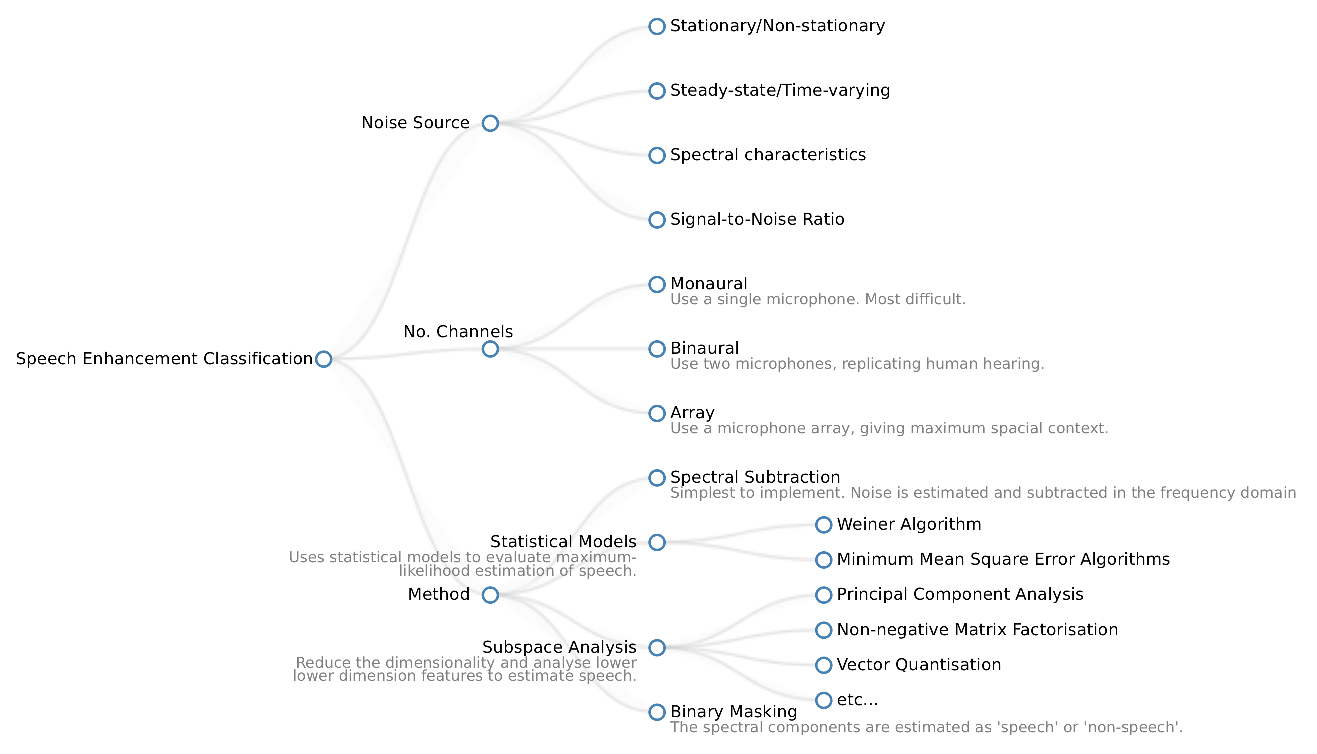
\includegraphics[angle=90,height=0.9\textheight]{fig/speech-enhancement-methods}\protect\caption{Some classifications of Speech Enhancement Methods\label{fig:Speech-Enhance-Classifications}}
\end{figure}



\section{Modelling Babble}

In a multi-speaker environment, and ignoring other forms of noise,
a signal can be considered a sum of multiple speakers:

\begin{equation}
X_{Babble}=\sum X_{Speakers}\label{eq:babble-sum-speakers}
\end{equation}


\nomenclature{$X$}{Short-time Fourier transform of a signal or recording, either with or without noise present. Rows represent frequency bins and columns represent time frames.}

(\ref{eq:babble-sum-speakers}) follows directly from the definition
of babble. The number of speaker signals used may vary, but to align
with with the definition for babble should be between three and six.


\subsection{For Generation}

It is generally desirable in testing to be able to present noise at
different \acp{SNR}. Rather than recording noise in a range of conditions
directly, it is more convenient to have separate speech and noise
and to model the speech with noise signal. Thus, the effects of babble
are often modelled rather than directly recorded. This type of babble
can be classed as synthetic babble, and may or may not accurately
represent real babble \citep{Krishnamurthy2009}.

The most common method of creating synthetic babble is to use a number
of speech recordings, adding them together to form babble. This presents
a number of issues. Firstly, real conversations are not simply a number
of voices speaking simultaneously. Rather, conversations are dynamic,
where there is generally one speaker but occasionally more or none
\citep{Krishnamurthy2009}. Secondly, synthetic babble generally does
not take into effect environmental effects, such as reverberation,
generally present alongside babble \citep{Krishnamurthy2009}.


\subsection{For Analysis and Enhancement}

For analysis, it is generally preferable to model a signal as a sum
consisting of a desired component and a noise component. The babble
model may exploit (\ref{eq:babble-sum-speakers}), such that a single
voice is modelled and extended to multiple speakers \citep{Mohammadiha2013a},
whereas other methods leave the model for babble as a generic noise
model \citep{Wilson2008}. The advantage of the latter is that the
same model may be applicable to other forms of noise.


\subsection{Separating Speech from Babble}

When the cocktail party problem was originally proposed, five factors
were identified as to how the human brain may differentiate between
the sources \citep{Cherry1953}, shown in \figref{Differentiating-Speech-Babble}
\vpageref{fig:Differentiating-Speech-Babble}.

\begin{figure}[h]
\centering{}\includegraphics[width=1\textwidth]{\string"fig/babble Separation\string".eps}\protect\caption{Differentiating Speech from Babble\label{fig:Differentiating-Speech-Babble}}
\end{figure}


Algorithms taking advantage of spatial differences and visual cues,
although effective \citep{Dupont2000}, require multiple channels
and visual data. Subspace methods take advantage of differences in
voices and differences in pronunciation. \ac{HMM} models for speech
recognition also take advantage of transitional probabilities \citep{Mohammadiha2013}.


\section{Methods for Evaluation of Speech Enhancement}

Methods for evaluating the intelligibility of speech, and by extension
speech enhancement, can be classified by the type of recognition they
measure: \ac{ASR} vs. \ac{HR}. This is necessary since \ac{ASR}
systems often recognise speech through a relatively low dimension
feature vector, whereas the human brain is far more sensitive. An
algorithm for enhancement may indeed improve the intelligibility for
an \ac{ASR} system, but side effects may be distracting or distortive
to a human listener.


\subsection{Human Recognition}

Intelligibility of a speech signal by humans is difficult to accurately
and quantitatively measure. The most obvious measure is to have human
test subjects listen to signals and judge which are more intelligible.
In order to achieve reputable, repeatable and accurate results a large
test is required with a large number of test subjects and recordings.

The \ac{ITU} standard for such tests is the \ac{MOS} \citep{InternationalTelecommunicationUnion1996}.
The test is designed to give an indication of the quality of telecommunication
transmission, but is applicable as a measure of speech intelligibility.
The \ac{MOS} results are a score calculated by the mean of the listeners\textquoteright{}
scores in the range one to five, with one representing the worst quality
and five representing the highest quality of intelligibility.

\ac{PESQ} is the \ac{ITU} standard for evaluation of objective speech
quality \citep{Rix2001,InternationalTelecommunicationUnion2001}.
This method provides an algorithm which estimates the improvement
quality by comparing a system\textquoteright s input and output \citep{Rix2001}.
Results show \ac{PESQ} scores give consistent and reliable estimates
on human perception, although are not directly comparable with \ac{MOS}
scores \citep{Rix2003}. Other methods for measuring perceptual quality
include long-term \ac{SNR}, segmental \ac{SNR}, weighted spectral
slope, log-likelihood ratio, Itakura-Saito distance, cepstrum distance,
\ac{SD}, \ac{SDR} and variations \citep{Hu2008}.


\subsection{Machine Recognition}

The most common technique to evaluate machine recognition quality
of speech is to run an \ac{ASR} algorithm on the signal and perform
a comparison of the \ac{WRR}. It should be noted that this method
is somewhat limited, in that different \ac{ASR} algorithms, which
may implement different feature vectors, may perform differently.
As such, results from different \ac{ASR} algorithms are not directly
comparable.

Algorithms in literature tend to limit evaluation methods to either
human recognition or machine recognition methods, as seen in \figref{Assessment-methods},
showing the evaluation measures used in various papers. This data
was gathered from the following papers \citep{Mohammadiha2013a,Wilson2008,Schmidt2006,Raj2005,Raj2005a,Raj2011,Fevotte2011}.

\begin{figure}[h]
\selectlanguage{english}%


\selectlanguage{australian}%
\centering{}\includegraphics[width=1\textwidth]{\string"fig/assessment Methods\string".eps}\protect\caption{Assessment methods used in literature\label{fig:Assessment-methods}}
\end{figure}



\section{Subspace Methods by Decomposition}

Subspace methods focus on reducing the dimensionality of a system.
This is done by decomposition or factorisation of a signal into lower
dimensional systems. Many techniques exist for decomposing a signal,
some of which are outlined in \figref{subspace-decomposition}.

\begin{figure}[H]
\selectlanguage{english}%


\selectlanguage{australian}%
\centering{}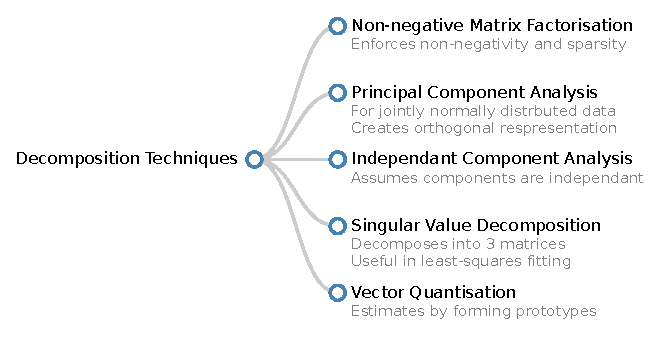
\includegraphics{fig/subspace}\protect\caption{Mathematical decomposition techniques for subspace analysis\label{fig:subspace-decomposition}}
\end{figure}


These techniques factorise a matrix into two matrix factors of the
form:

\[
C_{i\times j}\approx B_{i\times k}A_{k\times j}
\]


\nomenclature{$i$, $j$, $k$}{Matrix indexing placeholders.}

Often $k\ll i$ and $k\ll j$, meaning the factorised form may be
considered a more compact form.

\acf{NMF}, previously known as positive matrix factorisation, was
popularised by \citet{Lee1999} as a method lending itself to breaking
objects into their composing parts The distinguishing characteristic
of \ac{NMF} is that the product matrix, along with both its factors,
are non-negative, i.e. $A_{ij}\ge0,\, B_{ij}\ge0,\, C_{ij}\ge0\quad\forall\, i,\, j$.
\ac{NMF} has been demonstrated to be an effective method in dividing
images into parts \citep{Lee1999,Donoho2003}. Furthermore, \ac{NMF}
also has been shown to be useful on signals, specifically as a source-
separation algorithm \citep{Mohammadiha2013a,Wilson2008,Mohammadiha2013}.


\subsection{\acl{NMF} and Speech}

\ac{NMF} can be used in signal analysis, such that \citep{Lee1999,Paatero1994}:

\begin{equation}
X_{n_{f}\times n_{s}}\approx V_{n_{f}\times n_{c}}W_{n_{c}\times n_{s}}\label{eq:nmf-approx}
\end{equation}


where:
\begin{itemize}
\item $X$ represents the signal with rows of frequency bins results from
a Fourier transform and columns of time segments;
\item $V$ is the spectral components with columns representing typical
spectral vectors;
\item $W$ is the activation matrix, where each row represents the activation
levels of components at given times;
\item $n_{f}$ is the number of Frequency bins;
\item $n_{s}$ is the number of samples; and
\item $n_{c}$ is the number of components.
\end{itemize}
\nomenclature{$V$}{Spectral component matrix, one of the decompositions formed through the non-negative matrix factorisation procedure. Rows represent frequency bins and columns represent the component bases.}\nomenclature{$W$}{Activation matrix, one of the decompositions formed through the non-negative matrix factorisation procedure. Rows represent the component bases and columns represent time frames.}\nomenclature{$n_f$}{The total number of frequency bins.}\nomenclature{$n_s$}{The total number of time frames (samples).}\nomenclature{$n_c$}{The total number of component bases.}

\figref{nmf-on-speech} \citep{Mohammadiha2013} shows a visual representation
of this factorisation. It can be seen that the columns of the spectral
component matrix, $V$, represent approximations of the spectral components,
and that the activation matrix, $W$, is sparse.

\begin{figure}[h]
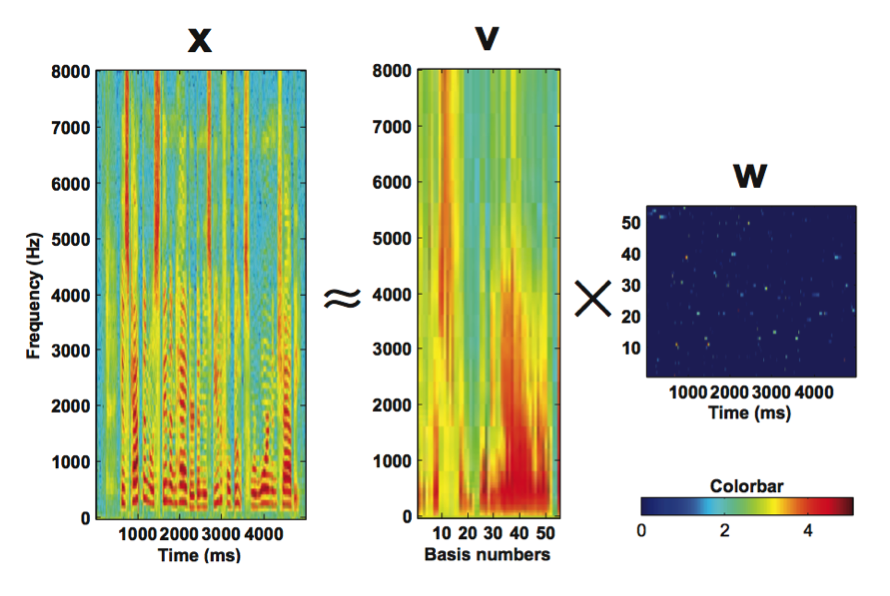
\includegraphics[width=1\textwidth]{fig/NMF-speech}\protect\caption{\acl{NMF} on speech\label{fig:nmf-on-speech}}
\end{figure}



\section{Assessment of Methods of Factorisation}


\subsection{Objective Functions}

\ac{NMF} algorithms aim to minimise or maximise an objective function.
The objective function is designed with an intent that optimisation
will ensure the approximation in (\ref{eq:nmf-approx}). The common
choice is to minimise the square error, or Euclidean distance between
$X$ and $VW$ seen in (\ref{eq:euclidean-distance-def}) \citep{Lee2000}.

\begin{equation}
F=\left\Vert X-VW\right\Vert ^{2}=\sum_{f=1}^{n_{f}}\sum_{s=1}^{n_{s}}\left[X_{fs}-\left(VW\right)_{fs}\right]^{2}\label{eq:euclidean-distance-def}
\end{equation}


\nomenclature{$F$}{The chosen objective function.}\nomenclature{$\Vert . \Vert ^2$}{Indicates the Euclidean distance.}\nomenclature{$f$}{Frequency bin index.}\nomenclature{$s$}{Time frame (sample) index.}

Another standard objective function based on the Kullback-Leibler
divergence of $VW$ from $X$ was proposed by \citet{Lee1999} and
is given as (\ref{eq:kl-divergence-def}). Here, the objective is
maximisation of the divergence objective function.

\begin{equation}
F=D_{KL}\left(X\|VW\right)=\sum_{f=1}^{n_{f}}\sum_{s=1}^{n_{s}}\left[X_{fs}\log\left(VW\right)_{fs}-\left(VW\right)_{fs}\right]\label{eq:kl-divergence-def}
\end{equation}


\nomenclature{$D_{KL}\left(.\right)$}{Indicates the Kullback-Leibler divergence.}

Often a modified objective function is used. This may add a cost function
in order to achieve auxiliary constraints \citep{Berry2007}. Some
examples of this are further discussed below. The objective function
is implemented using a series of update functions. The update functions
are iteratively processed until the approximation of $VW$ to $X$
is sufficient.


\subsection{Multiplicative Update Algorithms\label{sub:Multiplicative-Update-Algorithms}}

Updates are often implemented multiplicatively, since if all initial
matrices are non-negative and multiplications are positive, then the
final matrix will also implicitly be non-negative. This prevents the
need to explicitly enforce non-negativity. For the Euclidean distance
objective function, the multiplicative update rules are \citep{Lee2000}:

\begin{equation}
V_{fc}\leftarrow V_{fc}\otimes\left(XW^{T}\right)\oslash\left(VWW^{T}\right)\label{eq:mult-update-euc-v}
\end{equation}


\nomenclature{$\leftarrow$}{Indicates an iterative update rule.}\nomenclature{$\otimes$}{Element-wise multiplication.}\nomenclature{$\oslash$}{Element-wise division.}\nomenclature{$\left(.\right)^T$}{Matrix transpose.}\nomenclature{$c$}{Component base index.}

and:

\begin{equation}
W_{cs}\leftarrow W_{cs}\otimes\left(V^{T}X\right)\oslash\left(V^{T}VW\right)\label{eq:mult-update-euc-w}
\end{equation}


where $\otimes$ and $\oslash$ are the element-wise multiplication
and division operators. Alternatively, if the divergence objective
function is to be used,

\begin{equation}
V_{fc}\leftarrow V_{fc}\sum_{s}\frac{X_{fs}}{\left(VW\right)_{fs}}W_{cs}\label{eq:mult-update-div-v}
\end{equation}


and:

\begin{equation}
W_{cs}\leftarrow W_{cs}\sum_{s}V_{fc}\frac{X_{fs}}{(VW)_{fs}}\label{eq:mult-update-div-w}
\end{equation}


provide the required update rules \citep{Lee1999}. Additionally,
a third update rule \citep{Lee1999}:

\begin{equation}
V_{fs}\leftarrow\frac{V_{fc}}{\sum_{f}V_{fc}}\label{eq:mult-update-div-normalise}
\end{equation}


was included to normalise columns in the component matrix. This is
included to prevent continuously updating $V$ by a constant and $W$
by its inverse, which would otherwise be a valid update since $VW$
would be identical.

In addition, equivalent additive expressions can be formulated, known
as the gradient descent algorithms \citep{Lee2000,Berry2007}. In
this thesis, these forms are considered as equivalent \citep{Berry2007}
and thus are not considered separately.

The multiplicative update method of \ac{NMF} has been used extensively
in literature with good results \citep{Wilson2008,Raj2005}. However,
it has been shown that the proof given by \citet{Lee2000}, attempting
to prove the convergence of the multiplicative update rules (\ref{eq:mult-update-euc-v})
through (\ref{eq:mult-update-div-normalise}), was incomplete \citep{Berry2007,Finesso2006}.
The above equations may become stuck at stationary points and do not
always converge to the desired objective function \citep{Berry2007,Finesso2006,Finesso2004}.
When an element in $V$ or $W$ becomes zero it becomes \textquotedblleft locked\textquotedblright{}
and must remain as zero, an inherent flaw of the multiplicative update
functions \citep{Albright2006}. The following class of algorithms
allow flexibility in this respect.


\subsection{\acl{ALS} Algorithms}

\ac{ALS} algorithms are based on the initial proposed algorithms
by \citet{Paatero1994}. These algorithms are based on the alternating
variables method (or coordinate descent method) \citep{Wright1999}.
In these algorithms, first $V$ is fixed and $W$ is calculated using
a least squares method, then $W$ is fixed and $V$ is calculated
in a similar manner. These two steps are repeated until an adequate
approximation is achieved \citep{Albright2006}.

The least squares method used varies between \ac{ALS} algorithms.
\ac{ALS} algorithms can be generally classified by whether a non-negative
least squares method is used; or a general least squares method where
any negative values are subsequently set to zero. Non-negative least
squares methods converge to a local minimum successfully, however
the calculation cost per iteration is far higher despite attempts
to improve performance \citep{Berry2007,Albright2006,Lin2007,VanBenthem2004,Bro1997}.
General least squares methods may converge to a saddle point as opposed
to a minima. This is generally still preferred under practical conditions
due to the speed. Performance can also be improved by using a good
initialisation.

Typical \ac{ALS} algorithms \citep{Berry2007} using general least
squares method resemble the following:
\begin{enumerate}
\item Initialise $V$
\item Repeat the following for a predefined number of iterations:

\begin{enumerate}
\item Solve for $W$ using (\ref{eq:als-update-w}).
\item Set any negative elements in $W$ to zero.
\item Solve for $V$ using (\ref{eq:als-update-v}).
\item Set any negative elements in $V$ to zero.
\end{enumerate}
\end{enumerate}
\begin{equation}
V^{T}VW=V^{T}X\label{eq:als-update-w}
\end{equation}


\begin{equation}
WW^{T}V^{T}=WX^{T}\label{eq:als-update-v}
\end{equation}


The algorithms presented thus far present a common weakness in that
the update rules for the component matrix and the activation matrix
are the same (except that in some cases the component matrix also
has a normalisation update). This means there is little control over
which information is captured in the component matrix and which is
captured in the activation matrix.

The following algorithms are variations that attempt to provide further
control over ensuring that the components are completely captured
in the component matrix.


\subsection{Exemplar-Based \acl{NMF}}

This variation on the multiplicative update algorithm can be made
where it is expected that the components of the signal present themselves
individually, i.e. the signal is assumed to be a time series of components,
but with no simultaneous combinations of the components (this could
only be true for a single speaker). Here, the component matrix components
are drawn from the desired signal. This leaves only the activation
matrix to be calculated, so only one update rule is required, (\ref{eq:mult-update-div-w})
\citep{Raj2011}.

This is the case for clean speech signals, where bases are taken to
be phonemes \citep{Raj2011}. Taking advantage of this, phonemes may
be drawn randomly from speech and used to form the spectral component
matrix. The advantage of this method is that meaning is brought to
the components. This allows activations of a given component matrix
to be compared with those of another.


\subsection{Constrained \acl{NMF}}

Another method to ensure component information is captured within
the component matrix is to introduce sparseness constraints on the
activation matrix. By its nature, the activation matrix should be
sparser than the component matrix. Through the non-negative constraint
of \ac{NMF}, sparseness of the activation matrix (and indeed, also
the component matrix) naturally occurs \citep{Albright2006,Hoyer2004}.
However, it can be desirable to allow explicit control over the sparseness,
especially in speech applications \citep{Schmidt2006}.

\citet{Hoyer2002} proposed an algorithm based on the multiplicative
update algorithm in \citep{Lee1999} with an introduced cost function
to aid in control of the sparseness. This algorithm was further improved
in \citep{Hoyer2004} where the explicit control of sparseness was
introduced. This was achieved by defining the sparseness measure \citep{Hoyer2004}:

\[
sparssness(x)=\frac{\sqrt{n}-\left(\sum\left|x_{i}\right|\right)/\sqrt{\sum x_{i}^{2}}}{\sqrt{n}-1}
\]


Where $n$ is the length of vector $x$. The developed algorithm is
then based on the Euclidean distance objective function, employing
a combination of multiplicative update functions (�\ref{sub:Multiplicative-Update-Algorithms})
and gradient descent functions. However, the theory developed is applicable
to many types of objective functions and implementation algorithms
\citep{Cichocki2006}. Similarly, the cost functions introduced need
not be specific to sparsity, but can be applied to many auxiliary
constraints, such as enforcing smoothness \citep{Fevotte2011}.


\subsection{General \acl{NMF} approaches to Source Separation}

There are a number of methods to construct a clean-speech estimation
using \ac{NMF}. The particular methods used largely depend on the
specifics of the model used. However, the general concept is the same.
It is known that $X$ is approximated as $V\times W$ (\ref{eq:nmf-approx})
and therefore we can we can reconstruct a desired signal as:

\[
\hat{X}_{Desired}=V_{Desired}\times\hat{W}_{Desired}
\]


\nomenclature{$\hat{.}$}{Indicates an estimated value.}

Common algorithms form a component matrix for the desired speaker,
and another for the anticipated noise \citep{Schmidt2006,Raj2005,Wilson2008}.
These are concatenated, and the appropriate \ac{NMF} algorithms performed.
Afterwards, the speech-specific components can be separated again
and used to estimate the clean speech.

\begin{figure}
TODO DIAGRAM

\protect\caption{Common \acl{NMF} speech implementation}
\end{figure}


Limitations of these models mostly belong to the training, meaning
required \apriori{} knowledge. One issue is the required resources
for training, which can be upwards of an hour worth of recordings
\citep{Mohammadiha2013a,Raj2005}. Another issue is that these algorithms
are only effective for noise types that $V_{noise}$ has been trained
on, and thus have reduced flexibility.

\citet{Raj2011} proposed a different solution whereby an \ac{ASR}
system identifies phonemes in speech, and an \ac{NMF} algorithm is
implemented using one of 40 component matrices, one for each phoneme.
This model is somewhat limited in its application to babble, in the
author\textquoteright s opinion, as the initial \ac{ASR} algorithm\textquoteright s
performance is likely to be low on a noisy signal. However, the algorithm
did show that \ac{NMF} performance is be improved by forming bases
on phonemes. A novel alternative model was recently proposed by \citet{Mohammadiha2013a},
who used \acp{HMM} to form the basis of the \ac{NMF} algorithm separating
speech from noise , and thus used a temporally probabilistic method
to form and estimate of clean speech. By doing so, the algorithm accounts
for an extra feature outlined in \figref{Differentiating-Speech-Babble},
being the transitional probability.


\section{Summary}

The following three paragraphs outline the three proposed focuses
for this research.

Much work has been done in literature on speech enhancement under
noisy conditions. Systems are available to improve intelligibility
in telecommunication systems, or to improve the quality of \ac{ASR}
systems for home technology. However, most of the technologies outlined
in this literature review have not been implemented in end-user systems,
such as hearing aids or mobile technology. This is due to practicality
constraints within the algorithms, in particular the training requirement,
generally required to be specific to the end-user.

Additionally, most of the algorithms are tested for human recognition
improvements, but rarely for improvements in machine recognition,
highlighted in \figref{Assessment-methods}. Little literature exists
on the comparison of performance between these two forms of recognition.
An area of research proposed is to investigate the relationship between
human and machine recognition improvement under speech enhancement
algorithms, to see if one implies the other.

Finally, improvements have been made in focusing recognition by forcing
component matrices to represent phonemes. However, current algorithms
require complicated implementations. It is proposed to attempt to
simplify this process.\selectlanguage{english}%




\chapter{Methodology}

\acresetall

The algorithms outlined throughout the following chapter were implemented
in MATLAB. This environment was selected due to its availability and
ease-of-use. MATLAB includes a number of tools useful in signal processing
and statistical analysis \citep{Krauss1994,Jones1997}, and other
authors have provided tools in the MATLAB language \citep{Hoyer2004,Brookes1997,Loizou2008,Wojcicki2011}.
A limitation of the MATLAB environment in signal processing is the
comparative performance with lower-level languages, however performance
and speed were not a primary focus in this thesis, so this was deemed
acceptable.

Data analysis was conducted using R \citep{RCoreTeam2014}.

Simulations were run on a MacBook Pro 64-bit system with an Intel
Core i7 2.3GHz 4-core processor with 16GB memory, running OSX 10.9.2,
MATLAB R2013a and R version 3.1.0 (2014-04-10).

Test data to was drawn from the \ac{WSJ} corpus \citep{Robinson1995}.
Different recordings were reserved for testing and training. Babble
noise was simulated by using recordings of speech, also drawn from
the \ac{WSJ} corpus.


\section{Humanly Perceived Improvement vs. Machine Performance}

The first research area sought to answer research question \vref{enu:ResQ1},
\textit{\RQone{}} The focus was to compare and contrast the performance
differences of speech enhancement algorithms when evaluated on a human
listener versus a machine listener.


\subsection{\label{sub:Method-Existing-Data}Investigating Existing Data}

Data on enhancement performance of various algorithms and under different
measures of enhancement was collected from a number of sources \citep{mohammadiha2013supervised,Wilson2008,Schmidt2006,Raj2005,Rennie2008,Weninger2011,Williamson2014,Paliwal2010,Plourde2007}
and is presented in \chapref{Apx-Data}, \secref{litresults}. As
noted in \chapref{Literature-Review} \textit{\nameref{chap:Literature-Review}},
most literature takes preference to evaluation measures indicative
of either human performance or machine performance, but not both.
Thus, methods had to be developed in order to fairly compare the the
results between different sources.

The first comparison method was \textbf{direct comparison}. This method
involved plotting human performance against machine performance, and
thus was only applicable to a small subset of the results where both
performances were measured, such as in \citep{Paliwal2010}. This
data was analysed separately for each type of algorithm investigated.
Each data set had a \ac{LOESS} model fitted, in order to quickly
and visually judge the accuracy of applying a \ac{LM} fit. An \ac{LM}
model was then applied using R's \lstinline[language=R]!lm()! linear
regression function. The main limitation of the direct comparison
method was the limited dataset available.

A \textbf{grouped comparison} was also conducted. This was performed
as above, however similar algorithms were grouped into algorithm classes.
This allowed comparison of algorithm classes, to investigate whether
certain classes of algorithms are suitable for different purposes.

A limitation in these analyses is that the test conditions are not
fair: different noise types, subtle differences in algorithms, and
other differences could not be completely accounted for in the analysis.
As such, it was important to conduct further tests, where these conditions
can be controlled such that the comparisons be completely fair.


\subsection{\label{sub:Independent-Investigation-Meth}Independent Investigation}

Due to the lack of existing data on which conclusions can be drawn
on the human vs. machine success of various speech enhancement algorithms,
independent tests were required to be run. In order to answer the
research question, a number of enhancement algorithms were required
to be used to enhance speech, and a number of evaluation measures,
of both human perceptual and machine recognition types, were to be
used to measure the performance.

The Algorithms used in testing are given in \tabref{Algorithms}.

\begin{table}


\protect\caption{\label{tab:Algorithms}Algorithms used in testing}


\begin{tabular*}{1\textwidth}{@{\extracolsep{\fill}}|>{\raggedright}p{0.15\textwidth}|>{\raggedright}p{0.6\textwidth}|>{\raggedright}p{0.13\textwidth}|}
\hline 
Name & Description & Code\tabularnewline
\hline 
\hline 
Mohammadia Supervised & A supervised \ac{BNMF} algorithm proposed in \citep{mohammadiha2013supervised},
trained on simple utterances of the \ac{SoI}. & \lstref{mohammadiaSupervised}\tabularnewline
\hline 
Phoneme Mohammadia Supervised & A supervised \ac{BNMF} algorithm proposed in \citep{mohammadiha2013supervised},
trained on drawn phoneme samples of the \ac{SoI}. See \subsecref{Phoneme-Training}. & \lstref{mohammadiaSupervised}\tabularnewline
\hline 
Mohammadia Online & An online \ac{BNMF} algorithm proposed in \citep{mohammadiha2013supervised},
trained on simple utterances of the \ac{SoI}. & \lstref{mohammadiaOnline}\tabularnewline
\hline 
Phoneme Mohammadia Online & An online \ac{BNMF} algorithm proposed in \citep{mohammadiha2013supervised},
trained on drawn phoneme samples of the \ac{SoI}. See \subsecref{Phoneme-Training}. & \lstref{mohammadiaOnline}\tabularnewline
\hline 
Modified Supervised & A modified supervised \ac{BNMF} method using explicitly phoneme \ac{NMF}
bases. See \subsecref{Phoneme-Base}. & \lstref{modifiedSupervised}\tabularnewline
\hline 
Modified Online & A modified online \ac{BNMF} method using explicitly phoneme \ac{NMF}
bases. See \subsecref{Phoneme-Base}. & \lstref{modifiedOnline}\tabularnewline
\hline 
\acs{MMSE} & A spectral subtraction algorithm with \ac{MMSE} error estimation,
\lstinline[language=Matlab]!ssubmmse()! in \citep{Brookes1997},
trained on simple utterances of the \ac{SoI}. & \lstref{MMSE}\tabularnewline
\hline 
Phoneme \acs{MMSE} & A spectral subtraction algorithm with \ac{MMSE} error estimation,
\lstinline[language=Matlab]!ssubmmse()! in \citep{Brookes1997},
trained on simple drawn phoneme samples of the \ac{SoI}. & \lstref{MMSE}\tabularnewline
\hline 
Ideal Binary Mask & A ideal binary mask algorithm \citep{Wojcicki2011}, trained on simple
utterances of the \ac{SoI}. & \lstref{IDBM}\tabularnewline
\hline 
Phoneme Ideal Binary Mask & A ideal binary mask algorithm \citep{Wojcicki2011}, trained on simple
drawn phoneme samples of the \ac{SoI}. & \lstref{IDBM}\tabularnewline
\hline 
\end{tabular*}

\end{table}


The performance measures used were \ac{PESQ} \citep{InternationalTelecommunicationUnion2001},
\ac{MOS}, \ac{CCR} \citep{InternationalTelecommunicationUnion1996},
\ac{PRR} and segmental \ac{SNR}.


\subsubsection*{Objective Measures of Quality}

\ac{PESQ} was selected as a performance measure due to its extensive
usage in literature. Using the same evaluation measure allowed a certain
degree of comparability with others' results. The \ac{PESQ} implementation
used was a MATLAB implementation provided by \citet{Loizou2008}.

Segmental \ac{SNR} was also selected as a performance measure in
order to incorporate a statistical measure. A MATLAB implementation
was also supplied with \citep{Loizou2008}, so implementation was
straightforward.


\subsubsection*{Testing on Human Subjects}

\ac{MOS} and \ac{CCR} were selected due to their subjective qualities.
Although subjective measures are generally avoided, they were decided
to be useful in the experimental context, as human perception is itself
subjective. \ac{MOS}, like \ac{PESQ}, had been used throughout literature,
and so was included as a test measure for comparability. \ac{CCR}
was included also since the scale used lent itself to measuring enhancement,
and is in many ways more similar to \ac{PESQ} due to the fact it
measures improvement or degradation from a reference.

A MATLAB implementation of the \ac{MOS} test exists \citep{Ruzanski2009},
however the implementation was not flexible and the script was not
found to be suited to the required test. A new \ac{MOS} and \ac{CCR}
script was created, in alignment with the requirements outlined by
the \citet{InternationalTelecommunicationUnion1996}. The resulting
code is given in \Cref{lst:MOSScript,lst:MOS}, and has been submitted
to MATLAB Central and GitHub to share with the community \citep{Gillman2014}.

The scales used are given in \tabref{MOS-CCR-Scales}. Two \ac{MOS}
scales were used, one measuring quality opinion, and one measuring
required effort opinion.

\begin{table}[h]
\protect\caption{\label{tab:MOS-CCR-Scales}Scales used in subjective tests}


\begin{centering}
\subfloat[\acs{MOS} listening quality scale]{

\centering{}%
\begin{minipage}[t]{1\columnwidth}%
\begin{center}
\begin{tabular}{|c|c|}
\hline 
Quality of the speech & Score\tabularnewline
\hline 
\hline 
Excellent & 5\tabularnewline
\hline 
Good & 4\tabularnewline
\hline 
Fair & 3\tabularnewline
\hline 
Poor & 2\tabularnewline
\hline 
Bad & 1\tabularnewline
\hline 
\end{tabular}
\par\end{center}%
\end{minipage}}
\par\end{centering}

\begin{centering}
\subfloat[\acs{MOS} listening effort scale]{

\centering{}%
\begin{minipage}[t]{1\columnwidth}%
\begin{center}
\begin{tabular}{|c|c|}
\hline 
Effort required to understand the meanings of sentences & Score\tabularnewline
\hline 
\hline 
Complete relaxation possible; no effort required & 5\tabularnewline
\hline 
Attention necessary; no appreciable effort required & 4\tabularnewline
\hline 
Moderate effort required & 3\tabularnewline
\hline 
Considerable effort required & 2\tabularnewline
\hline 
No meaning understood with any feasible effort & 1\tabularnewline
\hline 
\end{tabular}
\par\end{center}%
\end{minipage}}
\par\end{centering}

\centering{}\subfloat[\acs{CCR} scale]{\begin{centering}

\par\end{centering}

\centering{}%
\begin{minipage}[t]{1\columnwidth}%
\begin{center}
\begin{tabular}{|c|c|}
\hline 
The quality of the second compared to the quality of the first & Score\tabularnewline
\hline 
\hline 
Much Better & 3\tabularnewline
\hline 
Better & 2\tabularnewline
\hline 
Slightly Better & 1\tabularnewline
\hline 
About the Same & 0\tabularnewline
\hline 
Slightly Worse & -1\tabularnewline
\hline 
Worse & -2\tabularnewline
\hline 
Much Worse & -3\tabularnewline
\hline 
\end{tabular}
\par\end{center}%
\end{minipage}}
\end{table}


When performing the \ac{MOS} and \ac{CCR} tests, some of the recommendations
could not be met. Sound-proof rooms were not available, as recommended
in \citep{InternationalTelecommunicationUnion1996} Annex A, and so
environmental, room and vehicle noise were not able to be tightly
controlled. However, an internal room, i.e., with no exterior walls,
was available. Measurements taken on a Samson Meteor condenser microphone
showed the environmental noise to be at an acceptable level, as seen
in \figref{Typical-noise-level}.

\begin{figure}
\begin{centering}
\includegraphics[width=0.8\textwidth]{fig/environment}
\par\end{centering}

\protect\caption{\label{fig:Typical-noise-level}Typical noise level during tests}
\end{figure}




The test setup is depicted in \figref{MOS-Test-setup}. The setup
was located in the aforementioned interior room. The test was performed
on a laptop running the MATLAB code (\lstref{MOSScript}), and the
test subject listened using a pair of over-ear headphones. Studio
quality headphones were not available, so Pioneer SE-MJ711 headphones
were used. The test procedure went as follows:
\begin{enumerate}
\item The subject was shown a recording of the \ac{SoI} so that they could
identify which speaker was the intended speaker in competing speaker
noise situations.
\item The test procedure was described to the subject, noting that three
separate tests were to be performed, meaning the subject would be
asked three types of questions.
\item With the laptop playing audio through the speakers, the test was begun
and the test coordinator showed the subject how to use the program,
running through approximately two iterations of the test.
\item The subject was then given headphones and instructed to start the
test.
\item The test coordinator was required to remain with the subject for the
duration of the test to answer any questions.
\end{enumerate}
\begin{figure}
\begin{centering}
\includegraphics[width=0.8\textwidth]{\string"fig/test setup\string".jpg}
\par\end{centering}

\protect\caption{\label{fig:MOS-Test-setup}MOS Test setup}
\end{figure}



\subsubsection*{\acl{ASR}}

Both \ac{HTK} and Sphinx were both considered for the \ac{ASR} system
for the \ac{PRR} results. Both offer comparable performance in recognition
and processing performance \citep{Vertanen2006}. \ac{HTK} was used
due to an availability of experience within the university. The chosen
\ac{ASR} method was a \ac{MFCC} feature vector. The selected training
data was the full recording set for the \ac{SoI}.

The script to implement the \ac{HTK} setup, training, extraction
and evaluation steps was based on that developed by \citet{Quill2014},
and is given in \ref{lst:ASR}. A basic overview of the script's function
is given in \algref{ASR}. The parameters used in performing the \ac{MFCC}
domain \ac{ASR} are given in \Cref{lst:MFC-config,lst:MFC-proto}.

\begin{algorithm}
\begin{enumerate}
\item Setup

\begin{enumerate}
\item Collate all test data into one folder, with a standard naming convention.
\item Produce required metadata on training data, including phoneme lists,
grammar rules, file lists, transcription summaries, etc.
\item Initialise empty initial \acp{HMM} using \ac{HTK}'s \lstinline[language=bash]!HVITE!,
based on a user defined configuration and prototype for the desired
feature vectors. In this case, these were those given in \Cref{lst:MFC-config,lst:MFC-proto}.
\end{enumerate}
\item Training

\begin{enumerate}
\item Convert training data to \ac{MFCC} domain using \ac{HTK}'s \lstinline[language=bash]!HCOPY!.
\item The \ac{HMM} model is then re-estimated twice, using \ac{HTK}'s
\lstinline[language=bash]!HEREST!.
\item The \ac{HMM} model is then re-estimated a further three times, this
time incorporating a short pause model but still using \lstinline[language=bash]!HEREST!.
\item The phoneme transcriptions are realigned using the current model and
\ac{HTK}'s \lstinline[language=bash]!HVITE!. The \ac{HMM} model
is then re-estimated yet another three times still using \lstinline[language=bash]!HEREST!.
\end{enumerate}
\item Extraction

\begin{enumerate}
\item Convert test data to \ac{MFCC} domain using \ac{HTK}'s \lstinline[language=bash]!HCOPY!.
\item Perform recognition and generate an estimated phoneme transcription
using \ac{HTK}'s \lstinline[language=bash]!HVITE!.
\end{enumerate}
\item Evaluation

\begin{enumerate}
\item Use \ac{HTK}'s \lstinline[language=bash]!HRESULTS! to compare the
estimated phoneme transcription with the original phoneme transcription.
\end{enumerate}
\end{enumerate}
\protect\caption{\label{alg:ASR} \acs{ASR} with \acs{HTK}}
\end{algorithm}


\begin{listing}[H]
\protect\caption{\acs{MFCC} configuration file\label{lst:MFC-config}}


\lstinputlisting[nolol=true,style=myBash]{../Code/python/MFC_HCompV_Config.ini}
\end{listing}


\begin{listing}[H]
\protect\caption{\acs{MFCC} prototype file\label{lst:MFC-proto}}


\lstinputlisting[nolol=true,style=myBash]{../Code/python/MFCProto}
\end{listing}



\section{Assessing \acl{NMF} Algorithm Training}

The second research area sought to answer research question \ref{enu:ResQ2},
\textit{\RQtwo{}} The focus was to investigate the training requirements
of supervised speech enhancement algorithms, and to investigate means
of improving the quality of training.


\subsection{\label{sub:Investigating-Training-Req}Investigating Training Requirements}

An experiment was conducted, investigating the effects of the performance
of enhancement. Firstly, test data was generated, using the code given
in \lstref{createTestData}, \textit{\nameref{lst:createTestData}}.
The data was formed as \lstinline[language=bash]!.wav! files consisting
of:
\begin{itemize}
\item training files, for use by supervised enhancement algorithms, for
both \ac{SoI} and noise recordings;
\item test files, or dirty files, for the enhancement algorithms to operate
on;
\item the clean file, for the evaluation algorithms to compare the enhancement
with; and
\item the clean noise file.
\end{itemize}
A range of training files were created, varying the number of utterances
included. The \ac{WSJ} corpus included 90 utterances per speaker%
\footnote{There are 90 utterances for the speakers reserved for training, \lstinline[language=bash]!si_dt!,
which were used in this test.%
} \citep{Fransen1994}, so 10 utterances were used for the test speech,
and the number of utterances used for training were varied between
1, 3, 5, 10, 15, 20, 30, 40, 50, 60, 70 and 80. The specific 10 utterances
used for testing were banned from being used for training to prevent
bias results.

Similarly, a range of test files were created by mixing a \ac{SoI}
recording with noise, varying the \ac{SNR}. The \ac{SNR} was varied
between -6dB, -3dB, 0dB, 3dB and 6dB. Additionally, a number of other
prerecorded noise types were drawn from the NOIZEUS corpus presented
in \citep{Hu2006}. The speakers used in each test are outlined in
\tabref{test-params}.

\begin{table}
\protect\caption{\label{tab:test-params}Simulations and associated parameters}


\begin{centering}
\begin{tabular}{|c|c|c|}
\hline 
Test Number & \ac{SoI} (sex) & Noise\tabularnewline
\hline 
\hline 
1 & C3C (f) & Competing speaker: C3F (m)\tabularnewline
\hline 
2 & C3L (f) & Competing speaker: C31 (m)\tabularnewline
\hline 
3 & C3S (m) & Competing speaker: C31 (m)\tabularnewline
\hline 
4 & C3S (m) & Synthetic babble: C31 (m) + C34 (m) + C35 (m)\tabularnewline
\hline 
5 & C3S (m) & Synthetic babble: C3F (m) + C3C (f) + C35(m)\tabularnewline
\hline 
6 & C3S (m) & Synthetic babble: C3F (m) + C3C (f)\tabularnewline
\hline 
7 & C3S (m) & Competing speaker: C3F(m)\tabularnewline
\hline 
8 & C3S (m) & NOIZEUS car\tabularnewline
\hline 
9 & C3S (m) & NOIZEUS babble\tabularnewline
\hline 
10 & C3S (m) & NOIZEUS street\tabularnewline
\hline 
\end{tabular}
\par\end{centering}

\end{table}


The enhancement algorithms used were those proposed by \citet{mohammadiha2013supervised},
two \ac{HMM} algorithms with \ac{BNMF} output distributions. One
uses a fully supervised method, and the other does not train for noise,
but estimates it online. The enhancement was conducted under all combinations
of utterances and \acp{SNR}. The code used to conduct the test is
given in \lstref{varyingTrainingTest}, \textit{\nameref{lst:varyingTrainingTest}}.

The performance of the enhancement algorithm was then analysed using
the \ac{PESQ} score, the \ac{PESQ} score improvement compared with
the dirty mixed signal, the segmental \ac{SNR}, and the segmental
\ac{SNR} improvement. The code used to perform this analysis is given
in \lstref{varyingTrainingAnalysis}, \textit{\nameref{lst:varyingTrainingAnalysis}}.


\section{\label{sec:Develop-Phoneme-Dependent}Developing a Phoneme-Dependent
Variation for the \acl{BNMF} Algorithm}

The performance of the \ac{BNMF} algorithm proposed by \citet{mohammadiha2013supervised}
was to be investigated when trained under a phoneme dependent context.
Two methods were proposed to achieve the phoneme dependence: firstly
leaving the training algorithm unmodified, but simply supplying training
data consisting of drawn phonemes, \textbf{\nameref{sub:Phoneme-Training}};
and secondly modifying the training algorithm itself to be phoneme
dependent, \textbf{\nameref{sub:Phoneme-Base}}.


\subsection{\label{sub:Phoneme-Training}Phoneme Dependent Training Data}

The first method of introducing phoneme dependence simply replaced
the typical recorded training data with a series of drawn phonemes.


\subsubsection*{Theory}

Typically, an \ac{NMF} algorithm is trained using utterances, either
from the \ac{SoI} or from a range of speakers, depending on the application.
However, it was noted that utterances were not an efficient method
of encapsulating the information relating to a voice. This conclusion
was drawn due to the fact that utterances contain redundant information,
as well as containing pauses that contain no information on speech.
It was also hypothesised that the training algorithms may be affected
by the inclusion of non-speech sections. The proposed method here,
of \textbf{phoneme dependent training data}, is intended to increase
the information density, such that the supplied training may be reduced
whilst still containing enough information to develop an adequate
model.


\subsubsection*{Implementation}

The drawn phonemes recordings were produced, the code for which is
included in \lstref{createTestData}, \textit{\nameref{lst:createTestData}}.
Phonemes were drawn randomly from the speaker recordings, and the
position in the phoneme is also randomly selected, i.e., drawn phoneme
samples are not always the beginning of the phoneme. The algorithm
used to produce drawn phoneme recordings is given in \algref{Producing-phoneme-training},
and the code in \Cref{lst:drawPhnSamples,lst:getSpeakerFiles,lst:getPhnData}.


\begin{algorithm}
\begin{enumerate}
\item Draw Phoneme Samples (\lstinline!drawPhnSamples.m!)

\begin{enumerate}
\item Read phoneme alignment (\lstinline!.phn!) file (\lstinline!getPhnData.m!)
\item For each possible phoneme

\begin{enumerate}
\item Shuffle the order of the phoneme occurrences in the alignment file
\item For each required sample (i.e. the number of samples being used for
each phoneme)

\begin{enumerate}
\item Select a random position within the occurrence of the phoneme
\item Record a sample of the required length
\end{enumerate}
\end{enumerate}
\end{enumerate}
\item Concatenate the samples and save \lstinline!.wav! file
\end{enumerate}
\protect\caption{\label{alg:Producing-phoneme-training}Producing phoneme training
data}


\end{algorithm}


The number of phoneme samples drawn and used was varied between 1,
5, 10, 50, 100, 500 and 999. The length of each sample drawn was $512/FS$,
so that 256 frequency bins were formed after taking the real \ac{FFT}.

Analysis was then performed similar to as described in \subsecref{Investigating-Training-Req}.
The \ac{SNR} was varied as before, and the online and supervised
algorithm variations \citep{mohammadiha2013supervised}, the \ac{MMSE}
algorithm \citep{Brookes1997}, and the ideal binary mask algorithm
\citep{Wojcicki2011} were tested using drawn phoneme training data.
The \textbf{phoneme dependent training data} enhancement algorithms
were tested against a all measures considered within this thesis:
\ac{PESQ}; \ac{MOS}, including listening effort and comparative
\ac{MOS}; \ac{PRR}, including correctness and accuracy; and segmental
\ac{SNR}.


\subsection{\label{sub:Phoneme-Base}Phoneme Dependent Base Matrix}

The second method proposed to use a completely phoneme dependent spectral
component matrix.


\subsubsection*{Theory}

In order to improve the previous algorithm, adaptations were proposed
to develop a phoneme-dependent method. It was assumed that speech
can be expressed as a sequence of phonemes, and that phonemes are
constant throughout their duration, such that a single speaker speech
signal may be expressed as:

\[
S=\left\{ p\left(1\right),p\left(2\right),p\left(3\right),...,p\left(T\right)\right\} 
\]


\nomenclature{$S$}{\ac{STFT} of a signal or recording of a single speaker.}\nomenclature{$p$}{The Fourier transform of a short recording of a single phoneme.}

where $S$ is the x\ac{STFT} of length $T$ and $p\left(t\right)$
is a single-frame \ac{STFT} of a single phoneme. Speech within babble
noise is of the form:

\[
X\left(t\right)=S_{1}\left(t\right)+S_{2}\left(t\right)+...+S_{N}\left(t\right)
\]


where $S_{1}\left(t\right)$ is the \ac{SoI} and other speakers $S\left(t\right)$
are competing speakers. It was assumed that, under this representation,
if $X$ were factorised using \ac{NMF} and the spectral component
matrix consisted of the phonemes present, that the activation matrix
would be a sparse matrix indicating which phonemes were present at
various times. \citet{Raj2011} demonstrated an increased separation
of speech from music when using phoneme-dependent separation, however
the algorithm used was more complex, involving online \ac{ASR} systems
to segregate phonemes before \ac{NMF} could occur during enhancement.
Here the segregation of phonemes is left as part of the \ac{NMF}
algorithm.


\subsubsection*{Implementation}

The proposed solution was to remove the training stage of both the
online and supervised methods, and allow the basis matrix to be directly
specified. This was achieved by modifying the \lstinline[language=bash]!NMF!
class supplied by \citet{mohammadiha2013supervised}, as given in
\lstref{NMF-train}, \textit{\nameref{lst:NMF-train}}. An alternative
to the existing \lstinline[language=bash]!train! function in the
\lstinline[language=bash]!NMF! class was implemented, \lstinline[language=bash]!dummyTrain!.
The simplified \lstinline[language=bash]!dummyTrain! allowed the
spectral component matrix%
\footnote{Variable name of the spectral component matrix in the in the \lstinline[language=bash]!NMF.m!
code is \lstinline[language=Matlab]!Et!%
} to be directly specified as opposed to trained.

This change was then utilised in both the online and supervised algorithms.
The phoneme training data (produced in \algref{Producing-phoneme-training}),
which was used also for the \textbf{phoneme dependent training data}
enhancement algorithms, was then read, made into a spectrogram, and
passed to \lstinline[language=bash]!dummyTrain!. The new algorithms
were called the modified online (\lstref{modifiedOnline}) and modified
supervised (\lstref{modifiedSupervised}) algorithms respectively.

In order to verify that the spectral component matrix was correctly
applied, the spectral component matrix \lstinline[language=Matlab]!speech_nmf.Et!
was returned and plotted.

Again, the \textbf{phoneme dependent base matrix} enhancement algorithms
were tested against a all measures considered within this thesis:
\ac{PESQ}; \ac{MOS}, including listening effort and comparative
\ac{MOS}; \ac{PRR}, including correctness and accuracy; and segmental
\ac{SNR}.



\chapter{Results}

\acresetall


\section{Humanly Perceived Improvement vs. Machine Performance}


\subsection{Investigating Existing Data}

The direct comparison method outlined in \subsecref{Method-Existing-Data}
was carried out on the data given in \secref{litresults} \textit{\nameref{sec:litresults}}.
The R code used to perform this analysis is given in \lstref{directComp}.

\figref{Direct-PESQ-PRR} shows the results obtained, comparing the
\ac{PESQ} improvement against the \ac{PRR} improvement. \figref{Direct-PESQ-PRR-LOESS}
shows the data fitted with an \ac{LOESS} model and \figref{Direct-PESQ-PRR-LM}
shows the data fitted with an \ac{LM} method.

\begin{figure}[p]
\subfloat[\label{fig:Direct-PESQ-PRR-LOESS}\acs{LOESS} fit]{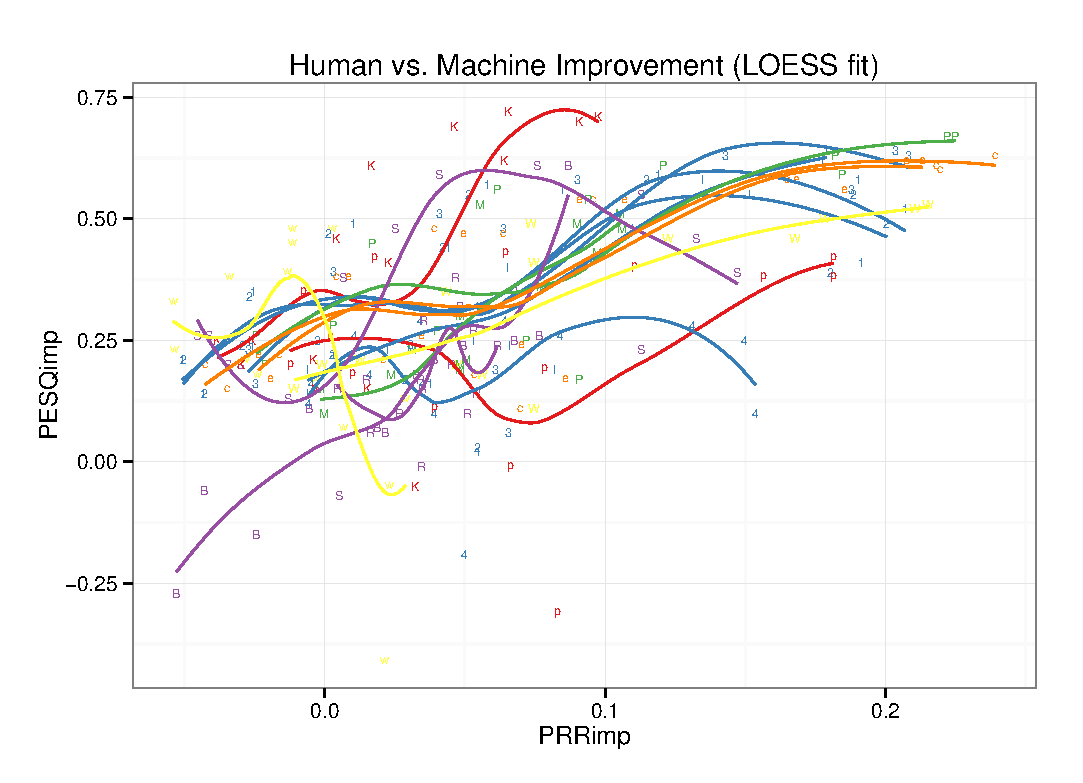
\includegraphics[width=1\textwidth]{fig/R/dir/HumanMachineAllLOESS}

}

\subfloat[\label{fig:Direct-PESQ-PRR-LM}\acl{LM} fit]{\includegraphics[width=0.8\textwidth]{fig/R/dir/HumanMachineAllLM}\includegraphics[width=0.2\textwidth]{fig/R/dir/HumanMachineAllLegend}

}\protect\caption{\label{fig:Direct-PESQ-PRR}Direct comparison of human (\acs{PESQ})
vs. machine (\acs{PRR}) quality improvement}
\end{figure}


Shown in \figref{Group-PESQ-PRR} are the results of the group comparison,
a method also outlined in \subsecref{Method-Existing-Data}.

\begin{figure}[p]
\subfloat[\label{fig:Group-PESQ-PRR-LOESS}\acs{LOESS} fit]{\includegraphics[width=1\textwidth]{\string"fig/R/dir/ HumanMachineGroupedLOESS\string".pdf}

}

\subfloat[\label{fig:Group-PESQ-PRR-LM}\acs{LM} fit]{\includegraphics[width=1\textwidth]{\string"fig/R/dir/ HumanMachineGroupedLM\string".pdf}

}\protect\caption{\label{fig:Group-PESQ-PRR}Grouped comparison of human (\acs{PESQ})
vs. machine (\acs{PRR}) quality improvement}
\end{figure}


Results outlined in \tabref{LF-Fit-Direct-Compar-PESQ-PRR} are the
coefficients relating to the \ac{LM} fitted lines in \figref{Group-PESQ-PRR-LM}.

\begin{table}[h]
\protect\caption{\label{tab:LF-Fit-Direct-Compar-PESQ-PRR}Summary of \acs{LM} fit
($y=mx+c$) of direct comparison of \acs{PESQ} vs. \acs{PRR} improvement}


\centering\csvautotabular{dat/HumanMachinePaliwal.csv}
\end{table}


Additionally, a Pearson's correlation table was formed over a number
of the evaluation measures, depicted in \figref{litResCorr}. In this
figure, the statistical evaluation methods are listed in blue, the
\ac{HR} methods are listed in red, and the \ac{MR} methods are listed
in green on the axes. The sparsity in this figure is due to the limited
amount of pre-existing data.

\begin{figure}[h]
\noindent \begin{centering}
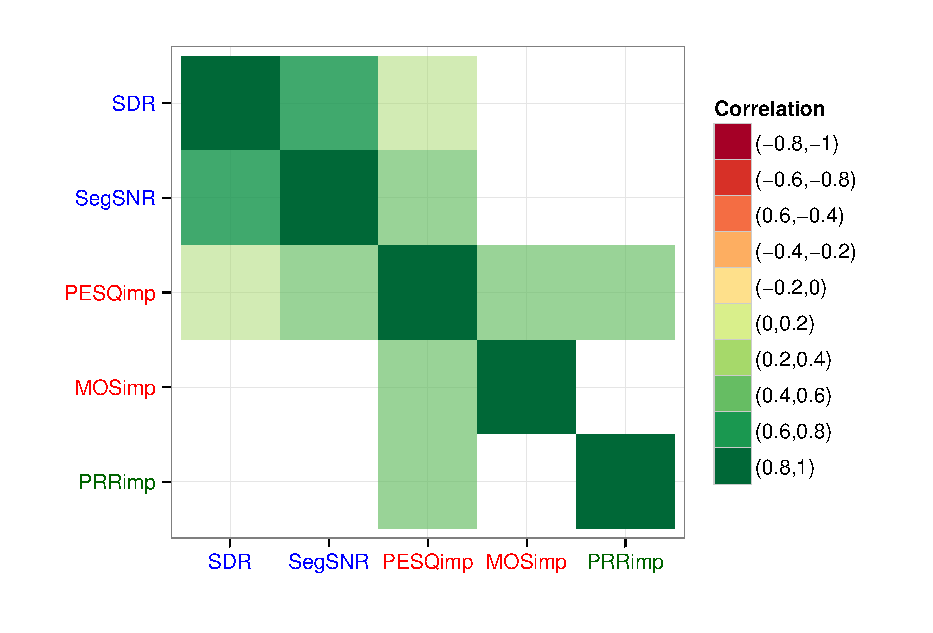
\includegraphics[width=0.7\textwidth]{fig/R/cor/litResCorr}
\par\end{centering}

Highlighted in \textcolor{blue}{blue} are the statistical measures,
\textcolor{red}{red} the human perceptual measures and \textcolor{dkgreen}{green}
the machine recognition measures.

\protect\caption{\label{fig:litResCorr}Pearson's correlation over some of the evaluation
measures assessed in existing data}
\end{figure}



\section{Assessing \acl{NMF} Algorithm Training}

The following are the results of investigations attempting to answer
Research Question \ref{enu:ResQ2}, \textit{\RQtwo{}}


\subsection{Investigating Training Requirements}

The results of the experiments proposed in \subsecref{Investigating-Training-Req}
are given in this section. \figref{vary-train-pesq} shows the \ac{PESQ}
results of the \ac{BNMF} algorithm developed by \citet{mohammadiha2013supervised}.
\figref{vary-train-pesq-imp} shows the \ac{PESQ} improvement as
compared to the dirty signal before enhancement. Similarly, \figref{vary-train-segsnr}
shows the segmental \ac{SNR} results of the same algorithm, and \figref{vary-train-segsnr-imp}
shows the segmental \ac{SNR} improvement compared against the signal
before enhancement.

Plots in \Cref{fig:vary-train-pesq,fig:vary-train-pesq-imp,fig:vary-train-segsnr,fig:vary-train-segsnr-imp}
each are arranged with the number of trained utterances on the x-axis
and test score on the y-axis. Furthermore, the plots are arranged
in a grid with rows corresponding to the enhancement algorithm and
columns corresponding to the test. Test labels give information on
the speaker ID and in brackets the sex of both the SoI, and the speakers
used to form the noise babble. Finally, series colour represents the
\ac{SNR} used for the test data, and the line type is dashed when
representing the score of the dirty signal before enhancement. The
R script used to form these plots is given in \lstref{trainReq}.

\figref{train-req-corr} shows a correlogram, an alternate view of
the same data. In the upper panels are scatter plots of each variable
pair. The lower panels are a heatmap of the Pearson's correlation
between the variables. Blue indicates a positive correlation, red
a negative, and the colour intensity indicates the magnitude.

\begin{figure}[p]
\noindent \begin{centering}
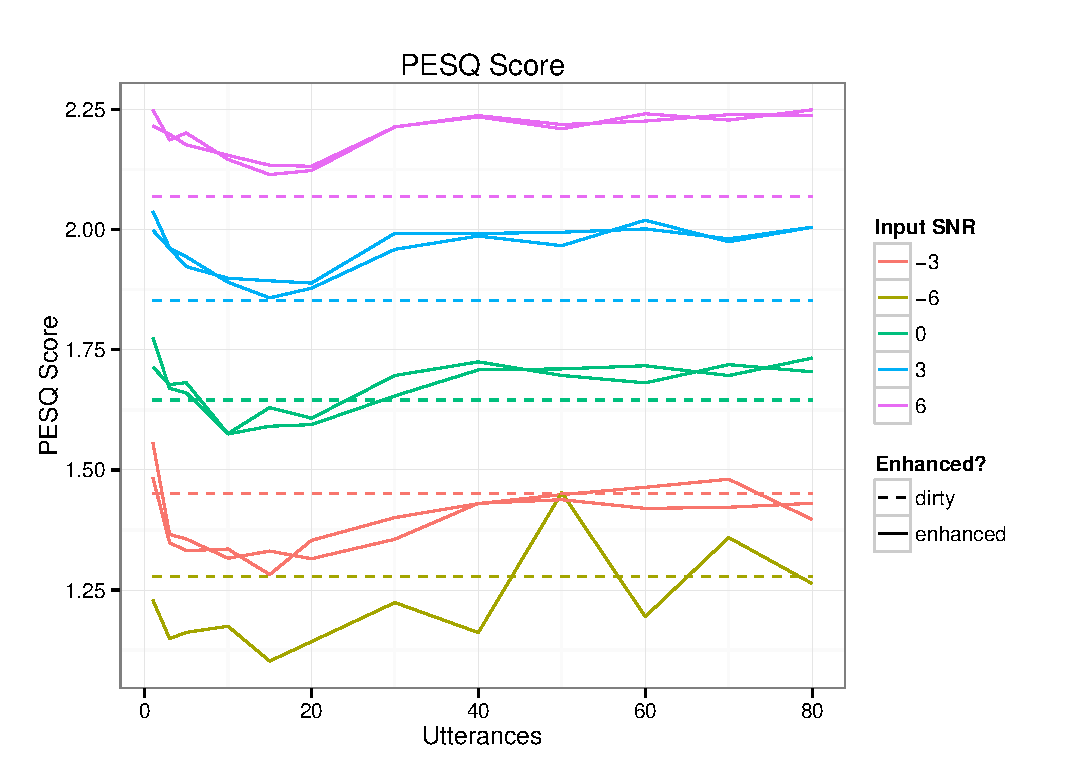
\includegraphics[angle=90,width=1\textwidth,height=0.95\textheight]{fig/R/train/pesq}
\par\end{centering}

\protect\caption{\label{fig:vary-train-pesq}\acs{PESQ} results of \acs{BNMF} algorithm
as training is increased}
\end{figure}


\begin{figure}[p]
\noindent \begin{centering}
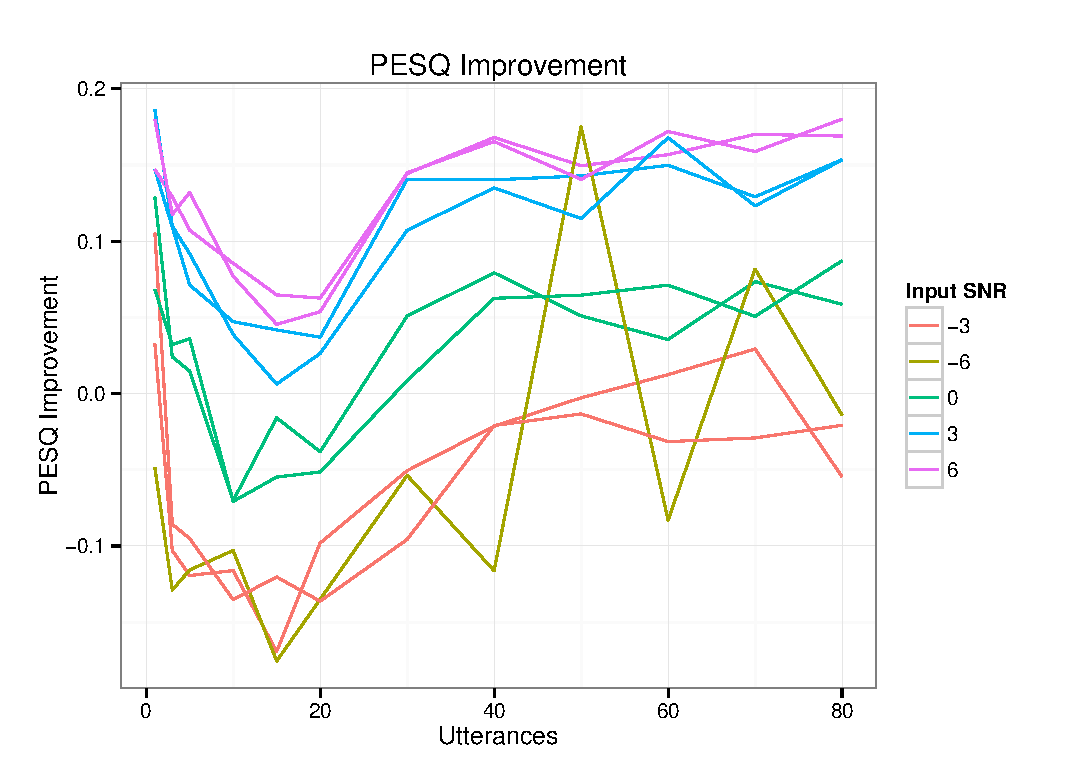
\includegraphics[angle=90,width=1\textwidth,height=0.95\textheight]{fig/R/train/pesqImp}
\par\end{centering}

\protect\caption{\label{fig:vary-train-pesq-imp}\acs{PESQ} improvement results of
\acs{BNMF} algorithm as training is increased}


\end{figure}


\begin{figure}[p]
\noindent \begin{centering}
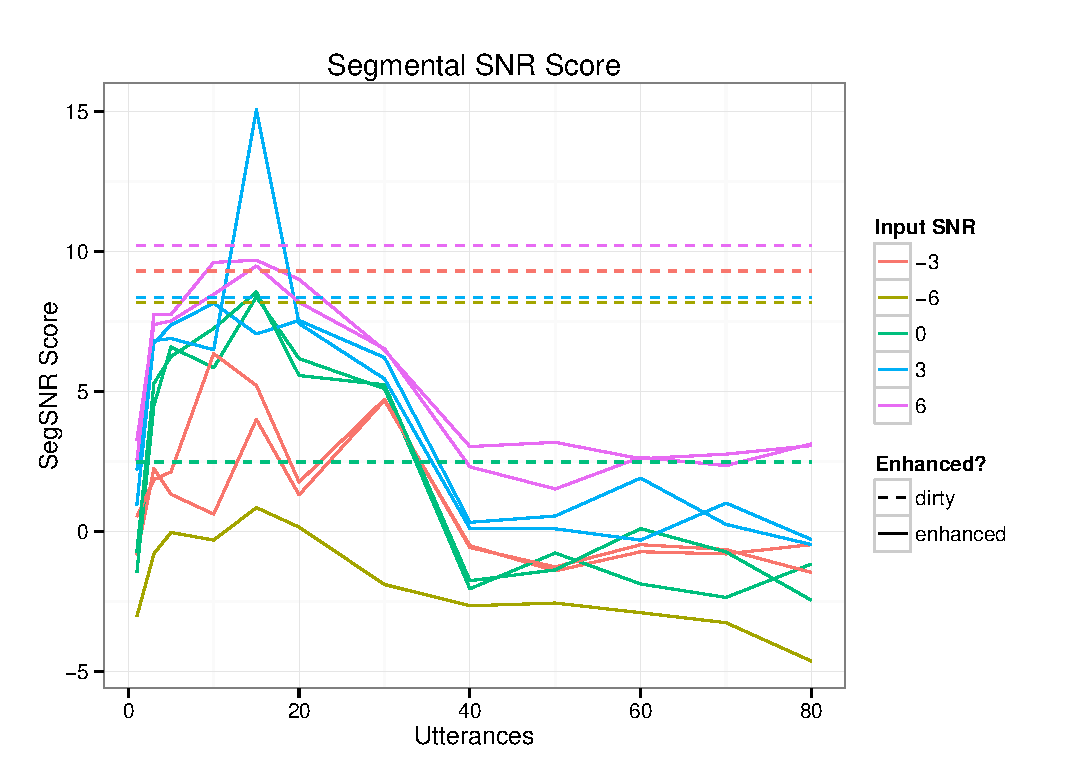
\includegraphics[angle=90,width=1\textwidth,height=0.95\textheight]{fig/R/train/segSNR}
\par\end{centering}

\protect\caption{\label{fig:vary-train-segsnr}Segmental \acs{SNR} results of \acs{BNMF}
algorithm as training is increased}
\end{figure}


\begin{figure}[p]
\noindent \begin{centering}
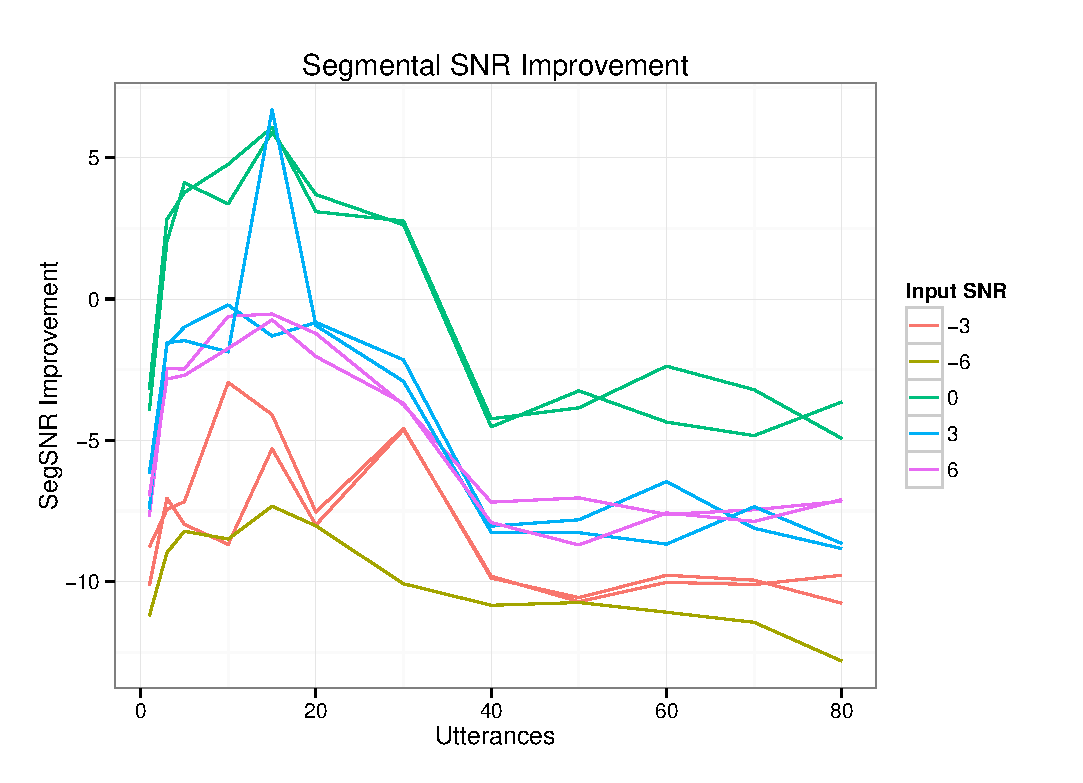
\includegraphics[angle=90,width=1\textwidth,height=0.95\textheight]{fig/R/train/segSNRImp}
\par\end{centering}

\protect\caption{\label{fig:vary-train-segsnr-imp}Segmental \acs{SNR} improvement
results of \acs{BNMF} algorithm as training is increased}
\end{figure}


\begin{figure}[h]


\noindent \begin{centering}
\includegraphics[width=0.9\textwidth]{fig/R/train/corr}
\par\end{centering}

\protect\caption{\label{fig:train-req-corr}Correlogram of results of training requirement
investigations}
\end{figure}



\section{Phoneme-Dependent Variation for the \acl{BNMF} Algorithm}

In order to force phoneme dependence in the algorithms to be modified,
phoneme samples first had to be formed. The phoneme sample recordings
were formed using the script in \lstref{createTestData}, with the
maximum number of samples drawn per phoneme varied. The length of
each sample drawn was $512/FS$, such that 256 frequency bins were
formed after taking the real \ac{FFT}. The typical spectrograms of
the drawn phonemes are given in \figref{drawn-phoneme-spectrogram},
showing the frequency characteristics of each phoneme.

\begin{figure}[h]
\subfloat[One sample per phoneme]{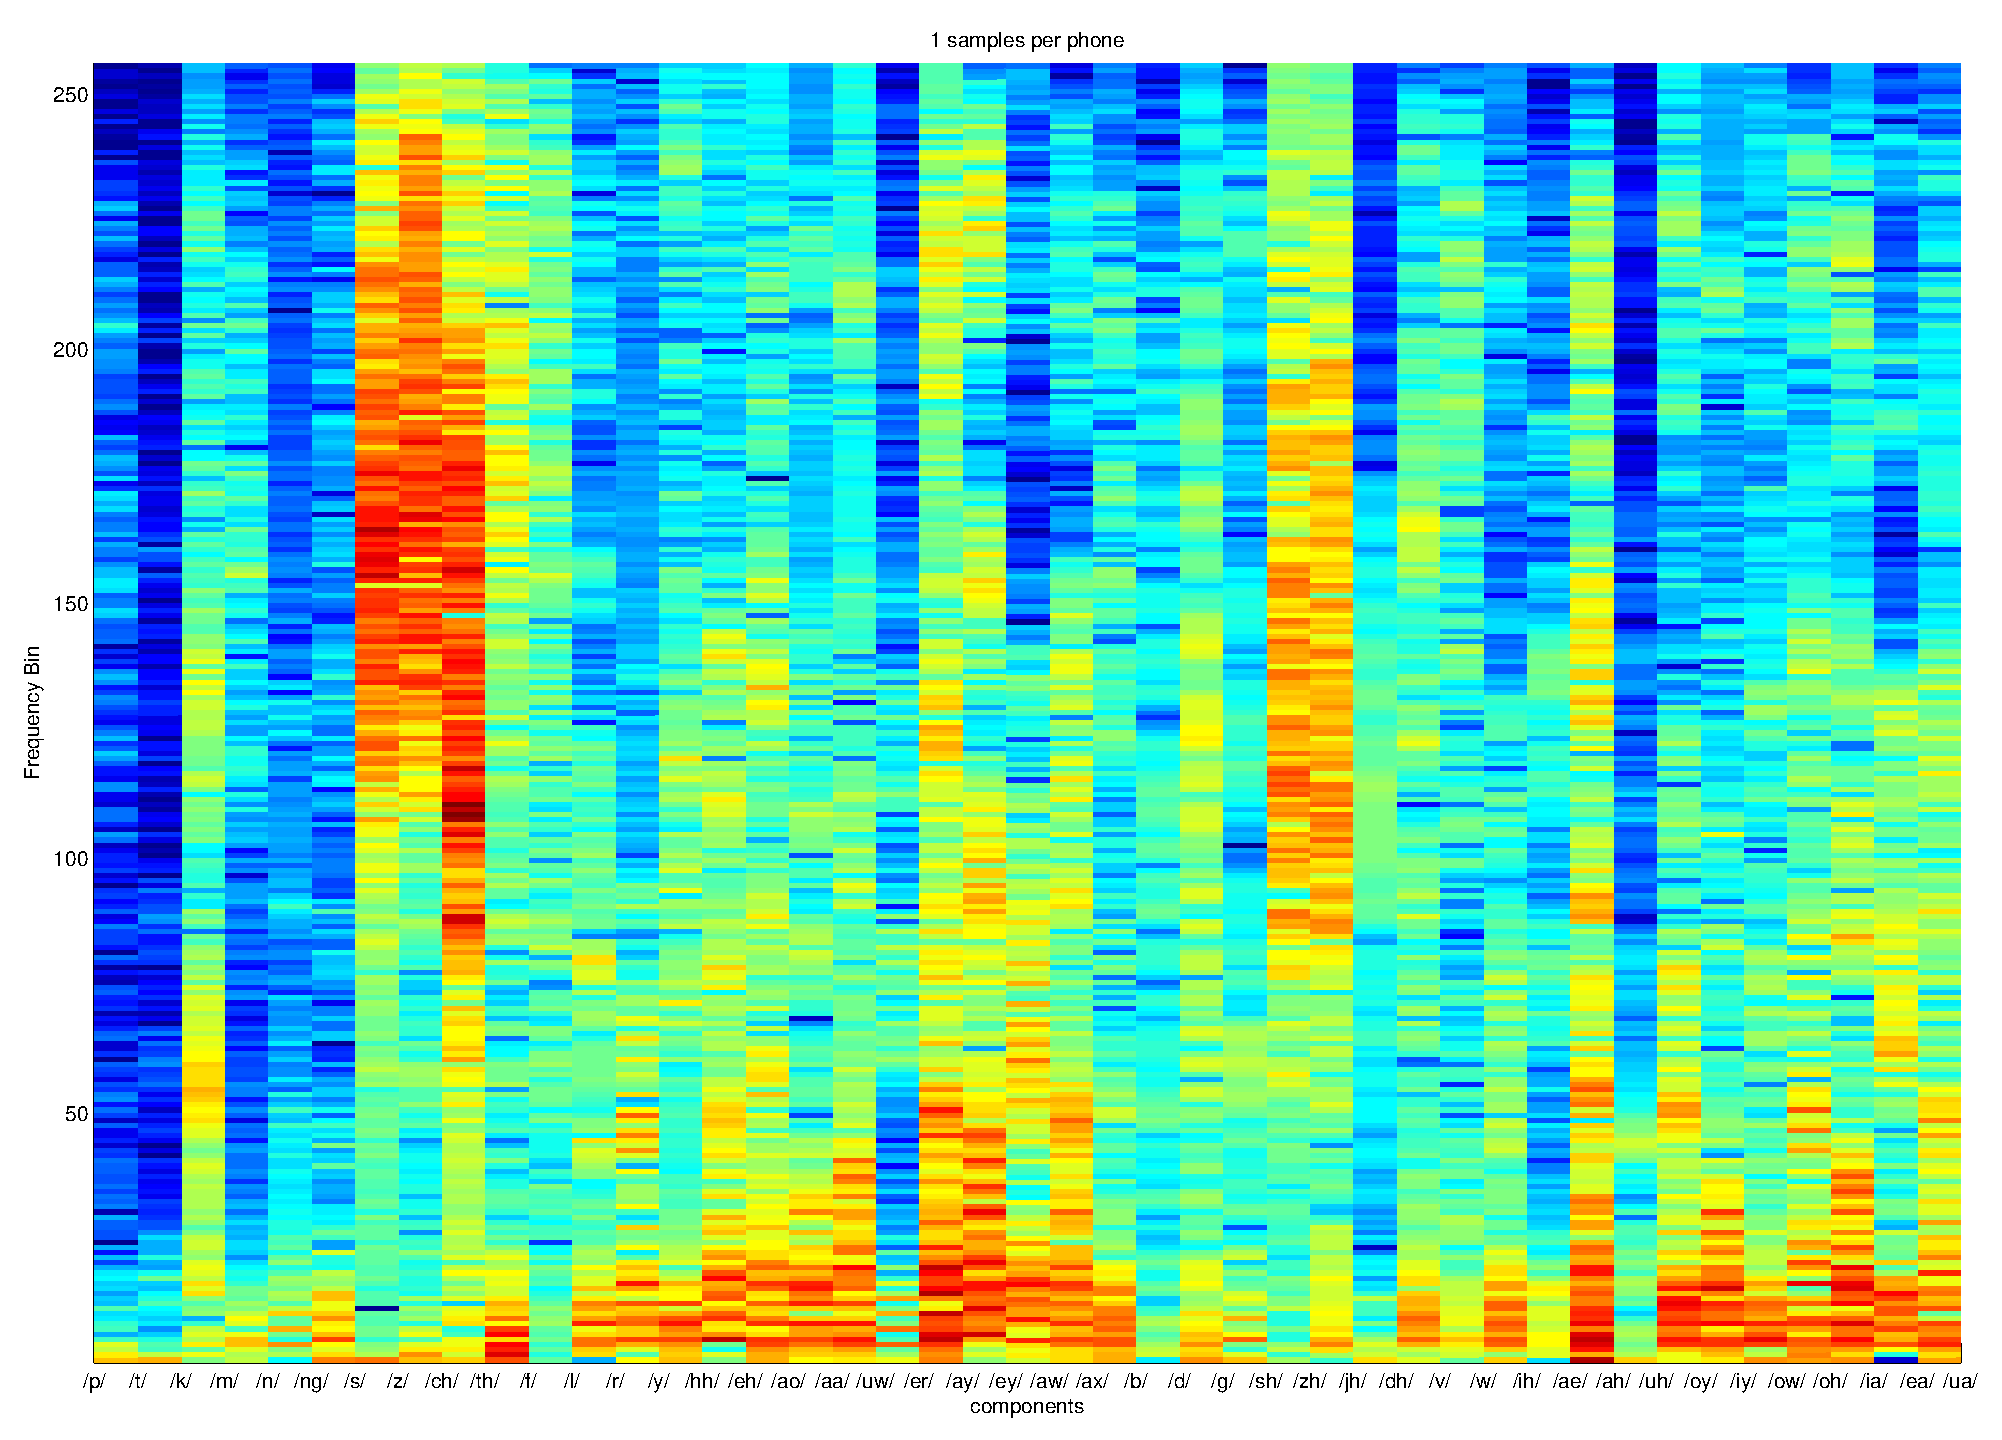
\includegraphics[width=0.5\textwidth]{fig/spectrogram/drawPhn/c3s-1phnSpectrogram}

}\subfloat[Five samples per phoneme]{

\includegraphics[width=0.5\textwidth]{fig/spectrogram/drawPhn/c3s-5phnSpectrogram}

}

\subfloat[Ten samples per phoneme]{\includegraphics[width=0.5\textwidth]{fig/spectrogram/drawPhn/c3s-10phnSpectrogram}

}\subfloat[50 samples per phoneme]{\includegraphics[draft,width=0.5\textwidth]{fig/spectrogram/drawPhn/c3s-50phnSpectrogram}

}

\subfloat[100 samples per phoneme]{\includegraphics[draft,width=0.5\textwidth]{fig/spectrogram/drawPhn/c3s-100phnSpectrogram}

}\subfloat[500 samples per phoneme]{\includegraphics[draft,width=0.5\textwidth]{fig/spectrogram/drawPhn/c3s-500phnSpectrogram}

}

\subfloat[999 samples per phoneme]{\includegraphics[draft,width=0.5\textwidth]{fig/spectrogram/drawPhn/c3s-999phnSpectrogram}

}

\protect\caption{\label{fig:drawn-phoneme-spectrogram}Typical spectrogram of randomly
drawn phoneme samples for speaker C3S}
\end{figure}



\subsection{Phoneme Dependent Training Data}

The following results relate to the proposed method outlined in \subsecref{Phoneme-Training}.


\subsection{Phoneme Dependent Base Matrix}

The first test conducted was to ensure the modifications to the code
indeed forced the \ac{NMF} spectral component matrix, \lstinline[language=Matlab]!Et!
in the \lstinline[language=bash]!NMF! class, to be the drawn phoneme
bases supplied.



\chapter{Discussion}

\acresetall


\section{Humanly Perceived Improvement vs. Machine Performance}

The aim of conducting research into existing data was to determine,
at a basic level, the correlation between \ac{HR} and \ac{MR}.


\subsection{Investigating Existing Data}

Results from conducting a direct comparison between \ac{PESQ} and
\ac{PRR} results were given in \figref{Direct-PESQ-PRR}. These results
show a general, positive correlation between \ac{PESQ} improvement
and \ac{PRR} improvement, and by extension between \ac{HR} and \ac{MR}.
The level of correlation appears to be relatively low, however comparison
with \figref{litResCorr} indicates the such levels of correlation
are expected. Indeed, similar correlations are observed between \ac{PESQ}
and \ac{MOS} results, which are both \ac{HR} measures.

\figref{litResCorr} Also indicates a very high correlation between
the raw \ac{PESQ} result and \ac{PRR}.

A number of further observations were drawn from \figref{Direct-PESQ-PRR},
and are highlighted in \Cref{fig:direct-klt-mband,fig:direct-klt-pklt,fig:direct-pklt-logmmse-spu-4,fig:direct-highcorr}.

Despite the high correlation between \ac{PESQ} and \ac{PRR} observed,
there is still evidence to show that algorithms' performances vary
depending on the performance measure used. For example, highlighted
in \figref{direct-klt-mband} are two algorithms, the \ac{KLT} method
and the \ac{MBAND} method, that exhibited similar performances when
evaluated by \ac{PRR}, a machine measure. However, when evaluated
by a human perceptual method, \ac{PESQ}, the \ac{KLT} method clearly
performed better. In fact, the \ac{KLT} method exhibited one of the
best performances seen on the \ac{PESQ} scale, whereas the \ac{MBAND}
method was the worst performer on this scale, exhibiting loss in perceptual
quality, as indicated by the negative performance.

\begin{figure}[h]
\noindent \begin{centering}
\includegraphics[width=0.8\textwidth]{fig/R/dir/lit/KLT-MBAND/HumanMachineAllLM}\includegraphics[width=0.2\textwidth]{fig/R/dir/lit/HumanMachineAllLegend}
\par\end{centering}

\protect\caption{\label{fig:direct-klt-mband}Direct comparison of \acs{PESQ} vs.
\acs{PRR} highlighting \acs{KLT} and \acs{MBAND}}
\end{figure}


\figref{direct-klt-pklt} shows the \ac{PESQ} vs. \ac{PRR} improvement
with the \ac{KLT} and \ac{pKLT} algorithm performances highlighted.
This was noted as an example of two very similar algorithms, with
varying performance between \ac{HR} and \ac{MR} results. The \ac{KLT}
results exhibited better performance for a human listener, as the
points laid higher on the y-axis, whereas the \ac{pKLT} results exhibited
better performance for a machine recogniser, as the points laid higher
on the x-axis.

\begin{figure}[p]
\noindent \begin{centering}
\includegraphics[width=0.8\textwidth,height=0.25\textheight,keepaspectratio]{fig/R/dir/lit/KLT-pKLT/HumanMachineAllLM}\includegraphics[width=0.2\textwidth,height=0.25\textheight,keepaspectratio]{fig/R/dir/lit/HumanMachineAllLegend}
\par\end{centering}

\protect\caption{\label{fig:direct-klt-pklt}Direct comparison of \acs{PESQ} vs. \acs{PRR}
highlighting \acs{KLT} and \acs{pKLT}}
\end{figure}


Such results support the proposition that some algorithms are inherently
suited either towards human or machine listeners. However, this shows
that such distinction is not necessarily related to the algorithm
class, since the \ac{KLT} and \ac{pKLT} algorithms belonged to the
same \ac{KLT} class, but produced different results.

The \ac{pKLT} and \ac{logMMSE-SPU-4} algorithms were observed to
show reasonable improvement in \ac{PRR} as the \ac{SNR} increased,
but little to no improvement in \ac{PESQ}. This is highlighted in
\figref{direct-pklt-logmmse-spu-4}, and is apparent by the near-zero
gradient. These algorithms likely introduce distortions into the signal
in the process of enhancement that the \ac{ASR} algorithm was immune
to, however would be distracting to a human and therefore performed
badly under the \ac{PESQ} evaluation.

\begin{figure}[p]
\noindent \begin{centering}
\includegraphics[width=0.8\textwidth,height=0.25\textheight,keepaspectratio]{fig/R/dir/lit/pKLT-logMMSE-SPU-4/HumanMachineAllLM}
\par\end{centering}

\protect\caption{\label{fig:direct-pklt-logmmse-spu-4}Direct comparison of \acs{PESQ}
vs. \acs{PRR} highlighting \acs{logMMSE} \acs{SPU} and \acs{pKLT}}
\end{figure}


The final observation drawn from \figref{Direct-PESQ-PRR} is highlighted
in \figref{direct-highcorr}, which shows the \ac{MMSE-SPU}, \ac{STSA-wcosh},
\ac{STSA-weuclid} and \ac{logMMSE-SPU-3} algorithms. These algorithms
show a high, positive correlation with one another, as well as exhibiting
the best results measured for both \ac{PESQ} and \ac{PRR}. The evidence
suggests such a response is the ideal case, and that there exists
algorithms which are capable of performing well for both human and
machine recognisers.

\begin{figure}[p]
\noindent \begin{centering}
\includegraphics[width=0.8\textwidth,height=0.25\textheight,keepaspectratio]{fig/R/dir/lit/MMSE-SPU-STSA-wcosh-STSA-weuclid-logMMSE-SPU-3/HumanMachineAllLM}
\par\end{centering}

\protect\caption{\label{fig:direct-highcorr}\acs{STSA-wcosh}, \acs{STSA-weuclid}
and \acs{logMMSE-SPU-3}}
\end{figure}


Results found using the grouped comparison method, shown in \figref{Group-PESQ-PRR-LOESS}
indicated that the data could be approximated by a linear model. The
\ac{LOESS} fitted lines were, in most cases, approximately linear.
The results for Wiener algorithms were a notable exception, with a
non-linear variation, even when the outliers are ignored. Overall,
the \ac{LM} fit in \figref{Group-PESQ-PRR-LM} is accepted to be
accurate.

The grouped linear fittings also correlate well with the best performing
individual algorithms, those highlighted in \figref{direct-highcorr}.

{*}{*}\textit{Conclusion, at the moment, is looking to be that in
general there is a good correlation between human and machine listener
improvement, and that, therefore, there will likely be many algorithms
suited to both purposes. However, still to warn that algorithms should
be verified both ways, as one does not imply the other.}


\subsection{Independent Investigation into \acl{HR} and \acl{MR}}

An independent investigation was conducted in which a number of enhancement
algorithms were implemented. The enhanced waveforms were then analysed
using a number of enhancement methods, covering both \ac{HR} and
\ac{MR}. The goal was to determine the correlation between evaluation
measures.

A summary of the correlation between all measurements made is given
in \figref{my-Corr}. A number of interesting observations were drawn
from this summary to be further investigated.

Firstly, it was noted that in \figref{my-Corr}, the correlation between
\ac{PESQ} and the various \ac{MOS} measures was low. This was a
surprising results as it has generally been determined in literature
that the two correlate well \cite{Kitawaki2007,Rix2003,Rix2001},
albeit with some exceptions \cite{Liu2006}. It was also noted that
the ideal binary mask algorithms performed very poorly overall on
the subjective scales in \Cref{fig:my-MOS,fig:my-MOSle,fig:my-CMOS}.
Furthermore, ideal binary mask algorithms had a very high variation
in \ac{PESQ} performance in \figref{my-PESQ}. Therefore, it was
suspected these results may be adversely affecting the overall correlation
between \ac{PESQ} and \ac{MOS}.

It was found that when the ideal binary mask algorithm data was omitted
the correlation between the \ac{PESQ} and \ac{MOS} increased, as
demonstrated in \figref{my-pesq-mos}. This indicated there were specific
occurrences for which the relationship between \ac{PESQ} and \ac{MOS}
demonstrated in literature do not hold.

\begin{figure}[h]


\subfloat[With the ideal binary mask]{

\includegraphics[width=0.4\textwidth]{fig/R/pair/my/pesq-mos}

}\subfloat[Without the ideal binary mask]{

\includegraphics[width=0.4\textwidth]{fig/R/pair/my/pesq-mos_no-IDBM}

}\includegraphics[width=0.2\textwidth]{fig/R/pair/my/pesq-mos_leg}

\protect\caption{\label{fig:my-pesq-mos}Scatterplot of \acs{PESQ} vs. \ac{MOS} results}
\end{figure}


The \ac{MOS} evaluation measures had a strong correlation with one-another
in \figref{my-Corr}, all at approximately 90\%. This was expected
between similar measures. However, it was noted that the same was
not true for the \ac{PRR} measures, where the correlation between
the correctness and the accuracy was found to be in general significantly
negative.


\section{Assessing \acl{NMF} Algorithm Training}


\subsection{Investigating Training Requirements}

The investigation to investigate training was conducted on two recently
proposed \ac{NMF} algorithms of interest, an online \ac{BNMF} and
a supervised \ac{BNMF}.


\subsubsection*{General Performance}

The algorithm performance was poor on the supplied test data. It can
be seen in \figref{vary-train-pesq-imp} that in general the enhanced
algorithm performed worse than the dirty recording, by the fact that
the improvement scores are predominantly negative. The algorithms
produced similar patterns consistently across tests, indicating it
is unlikely results are randomised outliers.


\subsubsection*{Online \acl{BNMF}}

Before tests were performed, it was hypothesised that increasing the
number of utterances provided as training would allow the algorithm
to produce a better model, with more data to learn from. However,
the number of utterances provided for training of the online \ac{BNMF}
algorithm in \figref{vary-train-pesq} had no significant impact on
\ac{PESQ} performance. In fact, a slight negative correlation may
be noted, which is supported by results in \figref{train-req-corr}.



\chapter{Conclusions}

\acresetall


\section{Humanly Perceived Improvement vs. Machine Performance}

In analysing the results gathered from literature, a strong correlation
between \ac{MOS} and \ac{PESQ} was found. Furthermore, a strong
correlation was found between \ac{PESQ} and \ac{PRR}, indicating
a correlation between \ac{MOS} and \ac{PRR}, thereby indicating
that in general, algorithms that are successful in \ac{HR} applications
are likely to be successful in \ac{MR} applications, and vice-versa.

Independent investigations supported the findings by directly comparing
\ac{MOS} results with \ac{PRR} results. A correlation was found
when the \ac{PRR} measure was an \ac{ASR} system's correctness.
However, a negative correlation was found when false insertions were
accounted for under the \ac{PRR}.

Furthermore, the ideal binary mask algorithm considered exhibited
a direct contrast with the general trend. The algorithm gave significant
improvements in reducing the noise, and therefore gave improvements
in the accuracy \ac{PRR}, indicating improvement for \ac{MR}. However,
the algorithm distorted the signal significantly, causing deterioration
in quality of \ac{HR}.

Thus it was determined that an algorithm's performance in enhancement
cannot be generalised over \ac{HR} and \ac{MR}.


\subsubsection*{Recommendation}

It is recommended that when enhancement algorithms are analysed, as
many evaluation measures be used as possible. Many of the evaluation
measures are relatively simple to use once implemented, and so the
cost associated with increasing the range of enhancement measures
is not large in the long term. An exception is the \ac{MOS} test,
which requires a considerable level of human time. The \ac{PESQ}
score may be used as a replacement, but the correlation between \ac{PESQ}
and \ac{MOS} in not certain.

In future work, it is recommended that the correlation between \ac{PESQ}
and \ac{MOS} be investigated under the context of speech enhancement
as opposed to measuring the quality of a telecommunications medium.


\section{Assessing \acl{NMF} Algorithm Training}


\bibliographystyle{bib/IEEEtranN}
\bibliography{IEEEabrv,bib/library}


\newpage{}

\appendix

\rfoot{}% no page no. in appendices}

\selectlanguage{australian}%
%\begin{landscape}


\chapter{\label{chap:Apx-Data}Data}


\section{Data Congregated from Literature\label{sec:litresults}}

%\includepdf[pages=-,angle=90]{dat/litresults}

%\end{landscape}

Just file ref?


\chapter{Code}


\section{MATLAB Test Code}

\lstset{style=Matlab-editor,basicstyle=\mlttfamily\small\singlespacing,title=\lstname}

\begin{listing}[H]
\protect\caption{Create Test Data MATLAB Code\label{lst:createTestData}}


\lstinputlisting[lastline=46]{../Code/MATLAB/Test/createTestDataBabble.m}
\end{listing}


\lstinputlisting[firstline=47,firstnumber=last]{../Code/MATLAB/Test/createTestDataBabble.m}

\begin{listing}[H]
\protect\caption{``Varying Training'' Test MATLAB Code\label{lst:varyingTrainingTest}}


\lstinputlisting[lastline=53]{../Code/MATLAB/Test/varyingTrainingTest.m}
\end{listing}


\lstinputlisting[firstline=54,firstnumber=last]{../Code/MATLAB/Test/varyingTrainingTest.m}

\begin{listing}[H]
\protect\caption{``Varying Training'' Analysis MATLAB Code\label{lst:varyingTrainingAnalysis}}


\lstinputlisting[lastline=53]{../Code/MATLAB/Test/varyingTrainingAnalysis.m}
\end{listing}


\lstinputlisting[firstline=54,firstnumber=last]{../Code/MATLAB/Test/varyingTrainingAnalysis.m}


\section{R Analysis Code}

\lstset{ language=R,% set programming language
         title=\lstname,
         basicstyle=\footnotesize\ttfamily\singlespacing,% basic font style
         keywordstyle=\color{blue},% keyword style
         commentstyle=\ttfamily\itshape\color{gray},% comment style
         numbers=left,% display line numbers on the left side
         numberstyle=\scriptsize\color{gray},% use small line numbers
         numbersep=10pt,% space between line numbers and code
         tabsize=2,% sizes of tabs
         showstringspaces=false,% do not replace spaces in strings by a certain character
%         captionpos=b,% positioning of the caption below
         breaklines=true,% automatic line breaking
         escapeinside={(*}{*)},% escaping to LaTeX
%         fancyvrb=true,% verbatim code is typset by listings
         extendedchars=false,% prohibit extended chars (chars of codes 128--255)
         literate={<-}{{$\leftarrow$}}1{<<-}{{$\twoheadleftarrow$}}1
         {~}{{$\sim$}}1{<=}{{$\le$}}1{>=}{{$\ge$}}1{!=}{{$\neq$}}1{^}{{$^\wedge$}}1,% item to replace, text, length of chars
         alsoletter={.<-},% becomes a letter
         alsoother={$},% becomes other
         otherkeywords={!=, ~, $, *, \&, \%/\%, \%*\%, \%\%, <-, <<-},% other keywords
         stringstyle=\color{dkgreen},
         deletekeywords={c, /}% remove keywords
}

\begin{listing}[H]
\protect\caption{Direct Comparison R Code\label{lst:directComp}}


\lstinputlisting[lastline=54]{../Code/R/directComp.R}
\end{listing}


\lstinputlisting[firstline=55,firstnumber=last]{../Code/R/directComp.R}

\begin{listing}[H]
\protect\caption{Indirect Comparison R Code\label{lst:indirectComp}}


\lstinputlisting{../Code/R/indirectComp.R}
\end{listing}


\begin{listing}[H]
\protect\caption{Training Requirement Comparison R Code\label{lst:trainReq}}


\lstinputlisting[lastline=60]{../Code/R/trainReq.R}
\end{listing}


\lstinputlisting[firstline=61,firstnumber=last]{../Code/R/trainReq.R}\selectlanguage{english}%


\end{document}
